%%%%%%%%%%%%%%%%%%%%%%%%%%%%%%%%%%%%
%
% pmx294.tex 1/22/2020
%
%%%%%%%%%%%%%%%%%%%%%%%%%%%%%%%%%%%%
\documentclass[11pt]{article}
%
\let\reft\ref
   \usepackage[dvips,colorlinks=true,linkcolor=blue]{hyperref}
   \usepackage[dvips]{graphicx}
   \usepackage{multicol}
%
\def\MusiXTeX{MusiX\TeX}
\def\bs{{\tt\char'134}}
\newcommand\PMXX{\textbf{PMX}}
\newcommand\PMX{\PMXX~}
\newcommand\IMA{\href{http://Icking-Music-Archive.org}{\underline{Icking Music Archive}}}
%
% Use \bfx for program names only.  Use \bf for single embedded letters 
%
\font\bfx=cmb10 scaled\magstephalf
\font\bfi=cmbxti10 scaled\magstephalf
\font\specfig=cmrj
\setcounter{secnumdepth}3
\setcounter{tocdepth}3
\def\Bslash{\tt\char'134}
\def\|{{\tt\char'174}}
\def\LBR{{\tt\char'173}}
\def\RBR{{\tt\char'175}}
\textheight= 9.5in \voffset-.8in%
\textwidth= 6.5in \hoffset-1.0in
\def\newfrom{2.59}  % changed every now and then 
\def\NEW#1{\ifdim#1 pt<\newfrom pt\else% 
\marginpar{\fbox{#1}}\fi}

\hoffset-54pt

%\let\rulet\rule\def\rule#1#2{\if#1<#2\rulet{.05in}{#2}\else\rulet{#1}{.05in}\fi} 

\begin{document}

\raggedright
\parindent24pt

\title{
  \Huge\bf
  PMX~--~a Preprocessor for \MusiXTeX{}\\
  \null\vskip-15pt
  \Large\sl
  Version 2.94~--~22 January 2020\\ 
  \author{\Large\rm Don \sc Simons\\
  \large\sl
  Dr. Don's PC and Harpsichord Emporium\\
  \normalsize\sl
  Redondo Beach, California, USA.\\
% To make the bitmapped eps: (1) TeX file with cmtt scaled 2500,
% (2) dvips -> gsview -> pdf.
% (3) gwin32 -sDEVICE=pnggray -sOutputFile=file.png -r100 -dEPSCrop -dbatch -q 
%    -dNOPAUSE -dTextAlphaBits=4 file.eps -c quit
% (4) file.png -> GIMP (crop out blank space) -> save as .eps.
%
  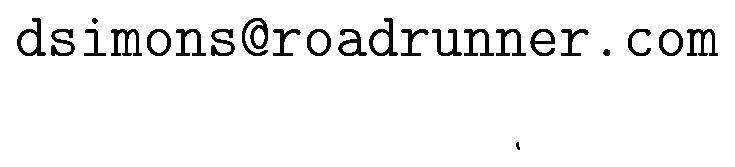
\includegraphics[scale=0.4]{file600.eps}}}

\date{}

\maketitle

\section*{Preface}
Compared to version 2.84, aside from bug fixes documented in the
opening comments in the source code, \PMX version 2.94 
enables blank gaps at the end or in the middle of a system (\ref{Gaps}),
allows virtually 
arbitrary staff jumping beams with multiplicity changes at the jump (\ref{Jumps}), 
allows 
changes to the vertical position of the number for a multibar rest (\ref{MultibarRest}),
and has more flexibility in setting stem lengths (\ref{Stemlength}).

\setcounter{page}1
% Need extra line to push last line of TOC to next page
~~
\tableofcontents
%\setcounter{secnumdepth}1
\pagestyle{headings}

%%%%%%%%%%%%%%%%%%%%%%%%%%%%%%%%%%%%%%%%%%%%
\def\boxitsep{10pt}
\let\hrt\hrule\def\hrule{\hrt height2pt}
\let\vrt\vrule\def\vrule{\vrt width2pt}
\def\boxit#1{\vbox{\hrule\hbox{\vrule\kern\boxitsep\vbox{%
\kern\boxitsep\hbox{#1}\kern\boxitsep}\kern\boxitsep\vrule}\hrule}}
\font\ded=cmssdc10 scaled \magstep3 
\bigskip
\setbox4=\vbox{
%  \hsize3in\noindent\strut 
  \hsize4in\noindent\strut 
     \centerline{\ded Dedication}
\vskip 3pt
The \MusiXTeX~community was stunned by the sudden death of Werner Icking on 
February 8, 2001.  He had been a benevolent patriarch, touching many 
of us not only
with his technical savvy and gentle guidance, but also his genuine kindness 
and generosity.  His spirit runs deep through all of \PMX.  His encouragement
fueled its development from its very beginning.  Many 
enhancements have been his proposals, including one he made on what
turned out to be his last day.  Werner, my friend, I dedicate this work to
you and your memory.  
}
\vfill
$$\boxit{\box4}$$
\let\hrule\hrt\let\vrule\vrt
\vfill
\eject

\section{Introduction}
%\setcounter{secnumdepth}1

        \PMX is a preprocessor for \MusiXTeX{}.  Before using it you should 
have installed \MusiXTeX~Version 1.21 \NEW{2.71} or higher, and 
any available version of \TeX~that includes e-\TeX.  The goal of \PMX is to 
facilitate the efficient typesetting of scores and parts
that have an almost professional appearance.  It can do {\it all} the work
involved in setting up {\tt \bs notes-\bs enotes} groupings, 
selecting groups of
notes to be beamed, defining beam heights and slopes, spreading the
entire piece evenly over specified numbers of systems and pages, and inserting
extra spaces where needed to make room for accidentals, flags, dots,
and new clefs. The input language for \PMX is much simpler than
\MusiXTeX.  You can enter note values and rests from 64ths to double 
whole notes ({\it breves}), ornaments, slurs, and limited text strings.  Every
voice in every bar must have exactly the correct number of beats in
the current meter, but you may change the meter at the beginning of any
measure, with or without printing the new time signature.  Before making a 
\TeX{} file, \PMX checks these timings and other aspects of the input.
\PMX has special features for dealing with baroque chamber music, including
the ability
to notate figured bass below the bottom staff in each system.  If \PMX hasn't
yet learned to do something you want to do, you can usually work around the 
problem by inserting literal \TeX\ strings in the \PMX input file.

     You can automatically create parts from a score using {\bfx scor2prt}.  
This auxiliary program generates a set of {\tt .pmx} input files, one for 
each part, from a single {\tt .pmx} file for the score.  
You can control the appearance of the 
parts with special commands in the main file, thereby making it  
possible to include within a single input file all the information 
that defines the score and the individual parts.

The basic \PMX
distribution as of this version of the manual is 
\href{http://icking-music-archive.org/software/pmx/pmx294.zip}
{\underline{\tt pmx294.zip}}.\NEW{2.94} It 
contains the FORTRAN sources, binaries that will run in a DOS
window on a PC with WINDOWS95 or higher, manuals for usage and for installation 
in DOS/Windows, and example typesetting files. Alternatively, the 
\href{http://www.icking-music-archive.org/software/htdocs/Getting_Started_Four_Scenar.html}
{\underline{software section}} of the Werner Icking Music Archive (WIMA) has instructions
for acquiring and installing \MusiXTeX~and \PMX on various platforms
(Windows, Mac-OSX, Unix-like systems) including using automated procedures from
several external \TeX~distribution sites.
The packages from those other sites will 
all eventually incorporate all the upgrades in {\tt pmx294.zip} but will take 
varying amounts of time to do so. \PMX is often upgraded; the most current version will
always be available directly from the ``News'' paragraph
\href{http://www.icking-music-archive.org/software/htdocs/htdocs.html}{\underline{here}}. 

\subsection{Conventions for This Manual}

	Hey, this is boring stuff, but if you take a minute to understand
the typographic conventions and a little jargon, 
it may avoid some confusion down the road.

	The typewriter typeface always indicates verbatim text as it would
be input to a computer.  This includes file names, \MusiXTeX{} tokens, and 
\PMX commands, e.g., {\tt barsant.pmx, \bs internote, c44}. 

	Bold is used for program names (e.g., {\bfx pmxab}), or when applied
to a single letter, to relate a \PMX command to its meaning (e.g., ``{\tt e}
signifies a l{\bf e}ft shift'').

        When\NEW{2.5}~viewing the PDF version of this document on a computer 
screen, clickable internal hyperlinks are colored blue, and clickable external 
links are underlined and colored cyan. 

        Italics may mean several different things depending on the context:
simple emphasis, or the first appearance of {\it jargon} 
(buzz-words that need to be explicitly defined), or finally  
to represent input variables for which some verbatim text would need to be 
substituted.  In the latter case the variable will be surrounded by
square brackets, e.g., [{\it basename}], but the brackets are not to be 
included with the substituted text.

        Speaking of jargon, there are several special words that have very 
specific meanings here: A {\it staff} is one set of 5 lines (plural 
{\it staves}), a {\it system} is a group of staves, and {\it voice} refers to 
one of the one or two 
simultaneous allowable sequences of notes in a staff. Note that this  
is a change \NEW{2.5}from versions prior to 2.5, where {\it voice} was used 
interchangeably with staff.

A \PMX {\it command} is a string of characters with no spaces between them. 
The first character determines the type of command. Any other characters 
are parameters that may be either required or optional. Sometimes we loosely 
use the word {\it command} to refer just to the initial character. 

\subsection{Setup}

	Here we briefly describe the setup for the Windows OS,
assuming \TeX\ and \MusiXTeX\ have already been installed. After compiling the
FORTRAN source code, users of other OS's 
may either adapt these instructions as needed or use one of the other setup 
methods referenced earlier. 

After decompressing the distribution file {\tt pmx276.zip}, 
you should have these 
files: \NEW{2.76} {\tt pmx276.for}, {\tt scor2prt.for}, two 
Windows executables {\tt pmxab.exe} and {\tt scor2prt.exe}, several sample 
{\tt .pmx} files,
{\tt pmx.tex}, {\tt ref276.tex} (\TeX\ source for a command summary),
{\tt pmx276.tex }(\TeX\ source for this file), 
PDF images of the latter two files, {\tt pmx25-276.html} showing 
changes from version 2.50 to 2.76, and {\tt install\_run\_PMX271.pdf} which gives more 
details about installing and running on different platforms.

%If necessary, compile the FORTRAN programs.
%I have tried to keep the source code as generic as possible, but minor 
%modifications may be needed for FORTRAN-to-C translation and/or other
%compilers.  

	Once you have assembled a full set of files, put the executables 
somewhere in the path or in your working directory, {\tt pmx.tex} into the 
texinput directory, the sample {\tt *.pmx} files in your working 
directory (the one from which you will run \PMXX), and the source code and 
document files wherevever you wish.

\subsection{Basic Operation, by Example}

Edit the 15th line of {\tt barsant.pmx} to contain the path to the 
directory where you want \PMX to write the {\tt .tex} file.  For example, 
if you want this to be the same as the working directory, type {\tt .\bs}~for Windows, 
or {\tt ./} for UNIX.   

If you haven't done so, open a command window and navigate to the 
folder containing {\tt barsant.pmx}. Execute \PMX by typing 
{\tt pmxab barsant} . Alternatively, you may 
just type {\tt pmxab <return>} and you will be prompted
for a jobname, which in this case is just {\tt barsant} .  
{\bfx pmxab} will always generate two files in the working 
directory: {\tt barsant.pml}
is a log file, and {\tt pmxaerr.dat} contains a single integer, 0 if 
the run was successful, otherwise the line number in the {\tt .pmx} file of the 
fatal error (useful for batch processing).   Also, on successful completion, 
{\tt barsant.tex} will be placed in the path specified in the setup.  

Now you are right where you would be after 
entering, debugging, and rough-editing the {\tt .tex} file manually.  To see 
the results, process {\tt barsant.tex} just as you would for any \MusiXTeX{} 
file, running all three passes, and view the {\tt .dvi} file, or go on and run 
{\bf dvips} to create a postscript file and view that with a postscript viewer
such as {\bf GSview}.  To make 
separate parts, run {\bfx scor2prt} by typing {\tt scor2prt barsant} .\NEW{2.0} 
The program will create a new {\tt .pmx} file for each instrument, in this
case {\tt barsant1.pmx} and {\tt barsant2.pmx}.
You may then process these 
files like you did the original one to create separate parts.

\section{Elements of PMX}
\def\l@subsection{\@dottedtocline{2}{5em}{20em}}%original 2 3.8 3.2
%\setcounter{secnumdepth}2

\subsection{Setup Data in the Input File} \label{setupdata}

	To see how the input file is put together, we'll look at 
{\tt barsant.pmx}.  For reference, here are are the first few lines:  
\pagebreak
\begin{verbatim}
%----------------%
%
%  barsant.pmx   Revised 29 June 2002
% 
%----------------%
%
% nv,noinst,mtrnuml,mtrdenl,mtrnmp,mtrdnp,xmtrnum0,isig,
  2    2      4       4        0      6      0       0 
%
% npages,nsyst,musicsize,fracindent
    1      7     20        0.07
Basso
Recorder
bt
./
\end{verbatim}
The lines 
with {\tt \%} in column 1 are comments.  
Some special handling of comment lines will be 
discussed in the section on creating parts from a score in  
section~\ref{scor2prt}.
   
The rest of the lines in this example are the {\it setup data}.  
Starting in the first non-comment line above,   

{\tt nv} (integer$\leq$24) \NEW{2.6} is the total number of 
sta{\bf v}es per system.  Each staff may contain either one or two voices,
but the total number of voices at any one time may not exceed 24.

{\tt noinst} (integer$\leq${\tt nv}) is number of {\it instruments}.  Each 
instrument has a unique name (see below), and any instrument
with more than one staff will have its staves joined with a curly bracket. 
Usually there is only one staff per instrument and {\tt noinst=nv}.  There
are two ways to assign more than one staff to one or more instruments. 
If only the first (lowest) instrument has more than one staff, such as in
a score for piano and a solo instrument, simply make
{\tt noinst$<$nv} and any difference will show up in instrument 1, the bottom
one in each system.  
\NEW{1.4} For a
more general distribution of staves among instruments, 
put a minus sign in front of {\tt noinst},
and follow {\tt noinst} with the number of staves in each  instrument  in
succession, separated by spaces.  These numbers must add up to {\tt nv} or your
computer will explode.  For a typical example of keyboard music, see 
{\tt mwalmnd.pmx}, in which {\tt nv=2} and {\tt noinst=1}, producing two 
staves per system with a curly bracket at the left.  

The number of instruments can be changed as well after the start of the 
score, but only to a number less than the original one.  See 
section~\ref{movbrk} to learn how to start with a smaller
number of instruments and later increase it.  

{\tt mtrnuml} is the {\it logical} numerator of the meter, or the number of 
beats per measure; {\tt mtrdenl} the denominator.  Please note the special
considerations in the paragraph after the next. If {\tt mtrnuml} is 
divisible by 2 or 3, beam grouping will be automatic; otherwise you will
have to force all beams using {\tt [}$\dots${\tt ]} as described in 
section~\ref{beams}.

{\tt mtrnmp} and {\tt mtrdnp} are the {\it printed} numerator and denominator.  
These determine the appearance of the meter in the printed output but 
have no effect on the internal timing analysis.  If {\tt mtrnmp$>$0} then it 
and {\tt mtrdnp} are printed literally as the numerator and denominator 
of the time signature.  Please note the special considerations in the following 
paragraph. If 
{\tt mtrnmp$<$0}, then the numerator is abs({\tt mtrnmp}) and the 
entire time signature will be printed with a vertical slash through 
it.  If {\tt mtrnmp}=0, then {\tt mtrdnp} determines the printed meter 
as follows: 

\medskip

\begin{tabular}{ll}
\tt 0 & No meter is printed ({\it blind} meter change)\\
\tt 1, 2, 3, or 4 & A single digit, between the 2nd and 4th lines\\
\tt 5 &  Cut time (alla breve)\\
\tt 6 &  Common time\\
\tt 7 &  Numeral 3 with a vertical slash\\
\end{tabular}

\medskip

There are special considerations for n/16 and n/1 time signatures (where the 
latter "1" normally means a whole note).  To get
n/1 time, use {\tt 0} (zero) for {\tt mtrdenl} and {\tt 1} for {\tt mtrdnp}.  To 
remember this rule, recall that the printed denominator is taken literally,
while the logical denominator can always be represented
by the same single digit used for the corresponding time value when entering 
ordinary notes (see section~\ref{notes}). So
for n/16 time, use {\tt 1} for {\tt mtrdenl} and {\tt 16} for {\tt mtrdnp}. 

If the first bar is a partial bar containing a pickup, {\tt xmtrnum0} is 
the number of beats in it; otherwise set it to 0.  It need not be an 
integer.  The first bar is the {\it only} bar that can have a different 
number of beats than the current value of {\tt mtrnuml} (Later we'll see how 
to change the meter).

{\tt isig} is the key signature, positive integer for sharps, negative for 
flats.

If {\tt npages}$>$0, it is the number of pages and {\tt nsyst} is the total 
number of systems in the entire piece.  \PMX will spread the entire 
piece horizontally over this number of systems, and vertically over 
{\tt npages} pages.  For proper vertical spacing there should be from 
about 9 to 16 staves per page.  If you specify too many staves for the number
of pages, one or more staves may spill over onto an extra sheet.  If this 
happens it will only become obvious when you preview the {\tt .dvi} file.  
One solution is to use the global option {\tt Ae} 
(see section~\ref{AeDirective}); another is to increase {\tt npages} or 
decrease {\tt nsyst}.

If {\tt npages} is set to 0, then {\tt nsyst} is interpreted as the average 
number of measures per system.  This is useful while building up a 
file a little at a time. \PMX will calculate how many systems to use, and
spread them over an appropriate number of pages.

{\tt musicsize} is 16, 20, 24, or 29, the height of a staff in points, with
20 considered the default\NEW{2.6}.

{\tt fracindent} is the indentation of the first system from the left 
margin, expressed as a decimal fraction of the total line width.

Next come the names of the {\tt noinst} instruments as you want them to 
appear within the indentation in the first system, one per line, 
starting with the {\it bottom} instrument.  If you've set {\tt fracindent}=0 
and don't 
want instrument names to appear, you must still leave {\tt noinst}
blank lines here.  Next comes a single string of {\tt nv} 
letters or numbers for the clefs, again starting with the bottom staff: 
\label{ClefCodes}
{\tt b,~r,~n,~a,~m,~s,~t,~f,~8} or digits 0-8 \NEW{2.71} respectively for {\bf b}ass, 
ba{\bf r}itone, te{\bf n}or, {\bf a}lto, {\bf m}ezzo-soprano, {\bf s}oprano, 
{\bf t}reble,\NEW{2.2} {\bf F}rench violin clef, or octave treble clef.   
The last line of setup data contains the path to the directory 
where you want the {\tt tex} file to go when \PMX creates it.  The one 
in {\tt barsant.pmx}~, 
{\tt ./}~, represents the current directory in UNIX and some versions of DOS.  
The path must terminate with {\tt /} or {\tt \bs}~.

\subsection{Structure of the Body of the Input File} \label{structure}

	The rest of the {\tt .pmx} file is the {\it body} of the input.  
The basic unit of input from here on is called an {\it input block} or 
just {\it block}, each one representing an integral number of bars.  If there
is a pickup bar defined by {\tt xmtrnum0} $>$ 0, 
it must be included in the first block {\it together with at least one full bar}. 
If you wish to put a pickup in a separate block, for example at the start
of a new movement, set the initial logical
meter to fit the pickup bar, then after the pickup bar do a blind meter change
as described in section~\ref{MeterChange}).

There will usually be 
4 to 8 bars in a block.  15 is the most allowed.  It is good practice 
to separate the blocks with comment lines that state which bars are 
represented, as I've done in {\tt barsant.pmx}.  
It is also advisable, although not required, to separate the bars with
the command {\tt |}. Its main functions 
are to provide visual separation in the input file, and to help isolate input
errors: if you put one anywhere except 
at a bar-end, {\bfx pmxab} will stop and show you where it detected the 
timing error. Otherwise, with several minor exceptions,
{\tt |} has no effect.  

At the start of each block there may be a few special commands 
(described starting in section~\ref{pmxcmds}).  
Next come the input data for the selected number 
of bars of the first (lowest in the system) voice in the first staff, followed by 
either {\tt /} to move to the next staff, or {\tt //} to move to the next voice 
on the same staff.  Each new voice must start on a new line 
in the input file, i.e., there should be no further data on the same input line
after {\tt /} or {\tt // }. 
   Continue entering other voices, each with 
{\it exactly} the same number of bars as the first, 
terminated by {\tt /} or {\tt //}, until
 the last (topmost in the system) ends with a {\tt /} and the block is 
finished.  Within 
a block every voice must have the same number of bars, but every block 
needn't have the same number of bars as other blocks.  The number of 
voices in a staff can only be 1 or 2, and cannot change within a block, but
may vary from block to block. 

	The data for each voice in each staff are a sequence of commands 
containing one or more adjacent characters.  Commands are separated from each
other by spaces.  The line-terminating commands {\tt /} and {\tt //} should also
naturally be preceded by a space.

\subsubsection{Notes} \label{notes}

	Commands for notes always start with a lower-case letter and, as 
with all commands, end at 
the first space. The first letter is the note name ({\tt a-g}).  The 
rest of the characters can be in any order with only a few 
restrictions.  The first digit defines the {\it basic time value} of the 
note: {\tt 9, 0, 2, 4, 8, 1, 3} or {\tt 6} respectively for double-whole,
whole, half, quarter, 
eighth, sixteenth, thirty-second, and sixty-fourth notes.  The second 
digit sets the octave (for reference, octave 4 runs from middle C to 
the B above).  Certain letters may appear after the initial one: {\tt d} 
for {\bf d}ot; {\tt dd} for \NEW{1.4} double dot; 
{\tt f, n,} or {\tt s} for {\bf f}lat, {\bf n}atural, 
or {\bf s}harp (repeat the letter  
immediately for a double); {\tt u} or {\tt l}, which  force the stem 
direction of any un-beamed note; {\tt e} or {\tt r} to shift the notehead 
l{\bf e}ft 
or {\bf r}ight by its own width; {\tt a} (for {\bf a}lone) which inhibits 
beaming for this note (or, if the first note of an xtuplet, for the
entire xtuplet); and \NEW{2.80}{\tt T} to insert a single-note {\it tremolo} 
on the stem (not to be confused with a 2-note tremolo, discussed later in 
section~\ref{TwoNoteT}). 
The {\tt T} may be followed by a single digit {\tt 1}, {\tt 2}, or {\tt 3} 
to indicate the
number of slashes in the tremolo symbol; {\tt 1} is the default if no digit
is entered. \NEW{2.4}A single accidental may be immediately 
followed by {\tt c} to
make it {\bf c}autionary, i.e., surround it with parentheses.
Alternatively, it may also be followed by {\tt i} to 
suppress typesetting \NEW{2.3} but still have 
the M{\bf I}DI processor honor the accidental.  Other characters allowed in note 
commands are {\tt +}, {\tt -}, {\tt .}(period), {\tt ,}(comma), {\tt x}, and 
several special characters following {\tt x}, all to be described below.  
Between the first letter and the end or {\tt x} if present,
non-digits can be in any order with respect to each other and to the digits, 
with minor exceptions involving shifting dots and accidentals.  

To move
a dot from its default location, simply follow the {\tt d}
with one or two decimal numbers, each predeced by 
{\tt +} or {\tt -}.  
The first is the 
vertical shift in \bs{\tt internote}s, the second, the horizontal shift in 
notehead widths.  

\label{AccidentalPosition}
Accidentals \NEW{1.4} can be shifted too.  One way is to enter 
{\tt +} or {\tt -} right after the accidental character, 
then an integer 
for the vertical shift, then another {\tt +} or {\tt -} followed by the 
horizontal shift in notehead widths.  If you use this method, you {\it must}
enter both numbers.  Or, to just shift horizontally, use
{\tt <} or {\tt >} followed by the shift in notehead widths.  When shifting
a sharp to avoid another sharp, a left shift of 0.85 is usually best.  When 
shifting a flat to avoid a flat above it, a left shift of 0.3 is suggested.
In chords (see section~\ref{chords}), if all the notes are in the same \NEW{2.4}voice, 
\PMX will automatically shift accidentals if required. This will be disabled 
for the current chord 
if any user-defined accidental shifts are entered, unless {\tt A} is entered 
along with the shift, e.g., {\tt zcsA<.5} . In that case the user-defined 
shift will be added to the PMX-computed one. 
\NEW{2.4} Another option that affects accidental positioning in 
chords is {\tt Ao},
entered in the main note command of a chord.  It will force the accidentals 
in that chord will be posted in the order
they come in the source file (starting with the main note), each one as far
to the right as it will go without crashing into a notehead, stem, or
another accidental. 


  Dots and accidentals always have to be entered when and if a note 
calls for them. i.e., they are never carried over from previous notes.  
On the other hand, the octave only needs to be entered if the note is 
more than a fourth away from the most recent note in the same voice.  
This feature lets you go for long stretches in a voice before needing 
to enter the octave.  An alternate way to jump more than a fourth but 
less than a twelfth is to type {\tt +} or {\tt -}.  In other words, these 
mean to put the note an octave higher or lower than it 
otherwise would have gone.  Two {\tt +}'s will raise the pitch two octaves 
above what it otherwise would have been, and so forth.  
The basic time 
value is also carried over from the past if it is not re-entered,   
except for the first note or rest in each voice in an input block, 
for which it {\it must} be entered.   
Therefore, when the melody jumps more than a 4th, using {\tt +} or {\tt -} is 
often more convenient than using a digit.  This is because in order to 
use the digit, you must first enter the basic time value whether it 
changes or not.  

	For example {\tt c44 d e f g a b c c0-} is an ascending quarter-note  
scale starting on middle C, followed by an octave jump down to a 
whole note middle C.  

	Explicit octave \NEW{2.1} numbers can be combined with one or
more {\tt +} or {\tt -} .  In earlier versions, {\tt +} or {\tt -} was
ignored if an octave number was specified.  This is a slight backward 
incompatibility; \PMX prints a warning when it happens.

\label{Stemlength}Stem length \NEW{2.73} can be {\bf s}hortened or {\bf l}engthened by {\it x} 
\bs{\tt internote} with the options {\tt S}{\it x} or {\tt L}{\it x}~. 
{\it x} is restricted to the range (0.5,4.0) for shortening and 0.5 to 27.5 
for lengthening.
The shortening can be made ``sticky'' by following the number {\it x} with 
{\tt :} . Then every note's stem in the voice will be shortened until 
one is encountered with the option {\tt S:} . By lengthening a stem enough 
to span to the next staff and connect with notes there, unflagged staff-spanning 
chords can be constructed. See section \ref{chords}~for further details 
about staff-spanning chords.

The first note command in each voice in a block must 
contain at a minimum the note name or {\tt r} for a rest (see below), 
and a basic time value.  For notes, it is good practice and can simplify 
editing
if in addition an explicit octave is set here.  However if it is not, 
\PMX will make some assumptions.  At \NEW{2.4} the start of the first 
input block the pitch will be set as if the prior note were middle C.
In later blocks \PMX will use the
obvious inheritance rules from the end of the prior block.  
However, if the number of voices in a staff  
has changed from the prior block, it is safest to reset the octave at the
start of a new block.  Duration is never inherited and must be set at the
start of each input block.   

	Dots can be a little tricky, because even though they affect the 
actual time value, they don't affect the basic time value, and it is only the
latter that is ``sticky".  Therefore, if a note is to be dotted, you always have to 
enter a {\tt d} (or a period, see next paragraph) somewhere within the 
command, after 
the note name, even if the actual time value and octave are the same 
as the prior note.  But the {\it basic} time value need not be re-entered if 
it hasn't changed (unless the note is more than a fourth from the 
prior note {\it and} you have for some strange reason elected to indicate the 
octave with a number rather than {\tt +} or {\tt -} ). So for example, 
consecutive dotted half notes, each within a fourth of the previous 
one, could be most cleanly entered as {\tt cd24 ed gd ed}, whereas {\tt cd24 e}
would represent a dotted half note followed by a plain half note 
(since the basic time value---as defined by the first digit---was a half 
note all along).

	There are two special shortcut rhythmic notations.  For normal dotted
rhythms (3:1 ratio), if you    
include a period ({\tt .}) in the note command, it will 
(a) assign a dot to the note just entered, (b) terminate that note, 
(c) prepare to 
receive the next note name {\it without any space}, and (d)~automatically 
assign a time value to the second note equal to one-third of the first one.
No time value may be entered for the second note, but octave and accidental
data may.  Ornaments and slurs (see below) following this command will apply 
to the second member. If you need to follow the main note 
with some modifying 
\NEW{2.3} 
command, you can still use the shortcut ({\tt .}) after that command and a
space. 
The main advantage of this shortcut comes if you want to 
follow one dotted pair with another of the same rhythm; then you 
needn't enter any explicit time value for {\it either} member of the second pair.  
This is possible because after using the shortcut,
the basic (inheritable) duration is set to that of the
{\it first} note in the pair, without the dot.

     For paired notes with 2:1 rhythmic ratios, the character {\tt ,}~(comma)
behaves similarly to the {\tt .}~(period) for 3:1 rhythms.

	Xtuplets, or groups of notes with their stems connected,
can have from 2 to 24 notes or\NEW{1.4} rests. Normally they
all have the same duration, but there are several options---described
below---to change this. The command for the first note of an xtuplet begins 
exactly like a 
note or rest command, with the name of the first note in the xtuplet, or
{\tt r} if it starts with a {\bf r}est (see subsection below on rests), 
and an optional time value.  
However, the actual time value (including a dot if present and a basic 
duration that may have been inherited from the prior note) now represents the 
{\it total} duration of the xtuplet.  Next (with no space, as usual) comes 
{\tt x} followed by either a one- or two-digit integer for the number of notes in 
the xtuplet, or \NEW{2.80}{\tt T} to initiate a 2-note tremolo, to be further
discussed below. The only options allowed immediately following the number are 
{\tt d} and {\tt n} . \NEW{2.4}{\tt d} signifies that the {\it first} note 
of the xtuplet should have a dot and the second, and extra flag.  
{\tt n} controls the printing of the {\bf n}umber and bracket. 
If {\tt n} is followed by a blank, then no number will be
printed. On the other hand, 
an \NEW{2.3}{\it unsigned} integer here is taken as a substitute number to
be printed instead of the natural one.  
If one or two {\it signed} decimal numbers follow {\tt n} 
(each starting with {\tt +} or {\tt -}), the first 
is a vertical shift in {\tt \bs internote}s, and the second, a horizontal shift 
in notehead widths. Another suboption to {\tt n} is {\tt f}, 
to {\bf f}lip the number vertically from its default position. A \NEW{2.5}final 
suboption to {\tt n} is {\tt s} followed by a signed integer. It applies only 
to non-beamed xtuplets, for which it tweaks the slope of the bracket above or 
below the xtuplet. For non-beamed xtuplets, you can further change the 
appearance of the bracket and number as explain in section~\ref{ATDirective}.

The second through last notes of the xtuplet are each then 
represented by a separate command containing a subset of the characters 
permitted for ordinary notes or rests: note name or {\tt r} (the only required 
character), accidental, and octave change character ({\tt +} or {\tt -}). 
\NEW{1.4} The octave may be given explicitly instead, and any integer will be 
interpreted as such, as no numerical time value is permitted.

To double\NEW{2.3} the duration of any note in an xtuplet, add the 
character {\tt D} to the command for that note. This will decrease the expected
number of notes in the xtuplet by one.  To add a dot to the doubled note
(as Bach sometimes did), use {\tt F} instead of {\tt D}.  
\NEW{2.4}To add a dot to one  
note and an extra flag to the next, include {\tt d} in the note command,
{\it after} the {\tt x} if it's the first note of the xtuplet as noted above.   

As an example, an ascending quarter-note triplet scale would be 
notated\hfil\break {\tt~c44x3~d~e~f4x3~g~a~b4x3~c~d~\dots} 

\subsubsection{2-note tremolos}\label{TwoNoteT}

A 2-note tremolo \NEW{2.80}is a special case of an xtuplet. 
It represent a rapid alternation between two notes. 
It is notated with a pair of 
notes, either beamed or unbeamed, with the possible addition of from one to three 
indented, disconnected beams between the two note stems. 
Like an ordinary
xtuplet, it begins with a note name, optional duration and octave, then
the character {\tt x}. The duration applies to the total time value of the 
two notes, is currently limited to either a half note ({\tt 2}), 
quarter ({\tt 4}), or eighth ({\tt 8}), and may be dotted by including~{\tt d}~after
the duration digit. 
Next comes a {\tt T}. This is optionally followed by one or two
integers from 0 to 3. The first indicates the number of ordinary beams 
connecting the two notes; the second, the number of indented beams.

The only other option allowed on the first note is to move the dot. After 
the~{\tt d}~enter one or two signed integers, where the first 
is a vertical shift in {\tt \bs internote}s, and the second, a horizontal shift 
in notehead widths. If the note has both a moved dot and a digit for an explicit octave, 
the~{\tt d} must follow the octave number

No other options are allowed, and some options are prohibited, such as zero
ordinary beams on anything except a quarter or dotted quarter tremolo. If no 
integers are entered after the~{\tt T}, defaults are assigned: (3,0) for a half, 
(0,3) for a quarter, and (1,2) for an eighth.  

After a space, the second note of the tremolo is entered. If the total duration 
is a half or dotted half, the 
noteheads will be open. For a whole note tremolo, two consecutive half note 
tremolos should be used. As with ordinary xtuplets, the horizontal spacing of the 
notes will always be the
correct value for notes with half the duration of the total. If the tremolo duration
is dotted, a dot will appear by default on the second note, and no~{\tt d}~should
be entered there unless the dot needs to be moved, in which case the syntax is as
described above for the first note.

Either\NEW{2.84} or both members of the tremolo may include chordal notes,
using the normal {\tt z} notation described in section~\ref{chords}. If the 
duration is dotted, dots will appear by default on chord notes, and again 
no~{\tt d}~should be entered there unless the dot needs to be moved.
If the tremolo is beamed, the height and angle of the beam may be adjusted
after making it a forced beam as described in section~\ref{beams}. 

Some examples of 2-note tremolos are shown below. When two versions are shown 
for a given duration, 
the first is the default. The following \PMX code generates the example.

~

{\tt f24xT a fxT a | fxT20 a fxT20 a /}

{\tt L2 fd24xT zefd-2+1 zcd-2+1 a r4 | f24xT a f2xT20 a /}

{\tt L3 fd44xT a r8 f44xT a  r4 | f44xT02 a fd8xT a r1 f8xT a r4 f8xT11 a /}

~

\includegraphics[scale=1.0]{tremxmpl4.eps}

\subsubsection{Rests}

	The command for a rest starts with {\tt r}.  
Then for a normal rest, in either order come a digit for the basic time value 
(using same codes as for notes, optional if unchanged from previous value),  
a {\tt d} if the rest is dotted, and a second {\tt d} if double dotted.
\NEW{2.0} The basic time value of a rest 
affects future notes and rests the same as if it had come from a note, 
i.e., it applies until another value is entered with a subsequent note 
or rest in the same voice.  The command {\tt rp} represents a 
full-bar rest notated with a {\bfi p}{\it ause} character (whole rest) 
regardless of 
the time signature; in this case no other duration information is 
needed or allowed.  {\tt rb}, followed if necessary by a duration 
specifier, denotes a {\bfi b}{\it lank} rest, one that occupies space and time 
but is invisible. This is most often used when there are
two voices in a staff and one drops out for some of the duration
of the current input block.  (See {\tt mwalmnd.pmx} for examples).  
\NEW{1.4} The 
option {\tt o} (for {\bf o}ff-center) suppresses centering a full bar rest.  If
you don't exercise this option, then 
{\it all} full-bar rests will be horizontally centered between bar 
lines, including pauses ({\tt rp}) as well as normal rests that fill the bar. 

	The default vertical position of a rest depends on whether there
are one or two voices in the staff. 
For one voice it is just the \MusiXTeX{} default 
(approximately centered on the middle line).  On the other hand, in  
the lower voice in 
a two-voice staff, the rest is lowered {\tt 4\bs internote}, while 
in the upper voice it is raised {\tt 2\bs internote}.  The \PMX default can be 
manually overridden by appending {\tt +}~or~{\tt -} and an integer 
representing the offset from the {\it middle} line of the staff 
(not from the \PMX default if there are two voices in the staff!).  
So for example, in a single staff 
in 3/4 meter, two voices, each with a half note followed by its own
quarter rest would be either 
\begin{verbatim}
c24 r4 //
c25 r4 / 
\end{verbatim}
or equivalently
\begin{verbatim}
c24 r4-4 //
c25 r4+2 / 
\end{verbatim}
while
\begin{verbatim}
c24 r4+0 //
c25 r4b /
\end{verbatim}
would produce two notes followed by a single, vertically centered rest.

Another way to override the default vertical positioning of rests is useful in
keyboard scores, or in fact any score containing two voices on a staff. 
The option {\tt K} (for {\bf K}eyboard) in the
{\tt A} command generally causes rests to be 
aligned horizontally with notes in the voice in which they are entered. See
section~\ref{Acommands} for a detailed description.

	\label{MultibarRest}The command {\tt rm} followed immediately by an 
unsigned integer will generate a {\bfi m}{\it ulti-bar} 
rest, a special combination of characters between two bar lines 
representing two or more bars of rest. The integer will always be printed, 
horizontally centered. The integer in the command \NEW{2.91}may optionally
be followed by {\tt n} and then another integer, possibly negative, indicating a
different vertical position for the number relative to the bottom staff line. 
The default is 9. To put the number
below the staff use -5 or -6. Once the height is changed it will stay the same until
changed again. The {\tt rm} command will generally only be used in separate parts 
that have been automatically generated by {\bfx scor2prt}. However, it
\NEW{2.4}may be used in a multi-line score, provided it is entered for the same
number of bars in every staff.

\subsubsection{Chords}\label{chords}

      Chordal notes, which always share a stem and the same time value as the 
prior note, are symbolized with {\tt z} (for {\bf z}ero time) followed by a note name and 
optionally an accidental, {\tt +} or {\tt -} as octave indicator, and {\tt e} 
or {\tt r} for a l{\bf e}ft or {\bf r}ight shift by one notehead width.
No basic time value is allowed.  If the main note
is dotted, then the chordal note will appear with a dot regardless of whether
a {\tt d} is entered.  The only time a {\tt d} is required in a chordal note
command is if the dot's position is to be adjusted; in this case the
{\tt d} is required, followed by one or two decimal numbers, each preceded by
{\tt +} or {\tt -}.  The first is the vertical shift in \bs{\tt internote}s;
the second, the horizontal shift in notehead widths. 
Any number of chordal notes can follow a 
single main note.  The stem direction of a chord is controlled by the main
note, but may be manually overridden with {\tt u} or {\tt l} in the main note
command.

    When chordal notes are beamed together, the default height and angle of 
the beam will be determined by the main note on each stem (the one without 
{\tt z}).  If a beam joining chordal notes looks bad, you can usually  
fix it either by changing which note acts as the main one, 
or by fine-tuning the beam parameters as described 
in section~\ref{beams}.

\PMX uses a complex algorithm to automatically position accidentals in chords. 
If you are unhappy with the result, you can manually tweak the horizontal 
positions as described in section~\ref{AccidentalPosition}.

Although there is no dedicated command for it, chords can be made to span from
one staff to another using various techniques\NEW{2.73}. The approach will depend on
whether 
the chord is single-stemmed with no flag, single-stemmed with a flag, or beamed. 
If beamed, it will also depend on whether it is an xtuplet or not. Examples of all
the basic possibilities are contained in the sample file {\tt staffcrossall.pmx}.  

For unbeamed, unflagged staff-crossing chords, 
by lengthening the stem with the {\tt L} option on the main note, it can 
be made long enough to join with an unflagged single-stemmed note or chord in the 
next staff. Single-stemmed notes with one or more flags can be joined across staves 
with a trick discovered by Andre Van Ryckeghem: In one staff create a standard note or 
chord with 
the stem pointing away from the other staff. In the other staff, place the chord notes
in a one-note forced beam that has been lowered or raised into the first staff
(e.g. {\tt [-10 b14 ]}); that
will stretch the stem to join the other notes, but with just one note (or chord) in the
beam, the crossbar will have zero length and be invisible. 

Beamed chords may also span from one staff to another, using joined beams (see 
section~\ref{beams}). The general approach is to construct a set of chords 
(or single notes, if the other chord notes are in the other staff) in each of
the two staves, enclose each set in a separate forced beam, and join the two 
beams with {\tt ]j}...{\tt [j}~. It is important to remember that the
lower staff is processed first. So in most cases, the end of the segment in the lower
staff must be joined (using {\tt ]j}) to the start of the upper segment (with {\tt [j}).
It turns out that for non-xtuplet beamed chords, in all cases where the chord at the 
beginning of the beam has a note 
in the {\it lower} staff, this works fine provided that the forced beams are of equal
duration and cover the same time span, and that positions in either staff with no note 
are represented with 
blank rests \bs{\tt rb} inside the force beam. So for example a set of beamed chords 
that starts only in the
lower staff and ends only in the upper could be represented by
\begin{verbatim}
[+28 g83 g g rb ]j /
[jf rb g84 g g ] /
\end{verbatim}
This example highlights some other issues, viz., that the beam height or direction of one 
or both beam groups may need to be altered. Often this will require trial and error. 

Unfortunately this two-group procedure breaks down if the first chord in the beam has no
notes in the lower staff. There are tricks to get around this; the user is referred to
the file {\tt staffcrossall.pmx} for examples. However, there is a much more 
straightforward way to define 
staff-crossing beamed chords that begin in the upper staff: it simply requires defining 
the beamed group in each staff as an xtuplet within a forced beam. It turns out that 
the treatment of 
staff-crossing beamed xtuplets is more robust than for non-xtuplets, and will admit
more intuitive coding. So for example, the reverse of the above example, where
the beam starts in the upper staff and ends in the lower, could be obtained with
\begin{verbatim}
[+28 rb2x4n g3 g g ]j /
[jf g24x4 g g rb ] /
\end{verbatim}
\newdimen\psav\psav=\parindent\parindent=0pt where we used the option {\tt n} to  
suppress printing the number. As you might expect, more general staff-crossing 
beamed chordal xtuplets follow the same concepts already described for non-xtuplets,
but as noted, they are more robust and admit patterns that start in the upper staff
and end in the lower one. {\tt staffcrossall.pmx} also contains examples this
approach.
 
\parindent=\psav

\subsubsection{Grace notes}\label{graces}

	A grace note command starts with a {\tt G}.  It is entered in its natural
order, normally before the main note, but sometimes after.  After {\tt G} and
before the note name, comes any 
combination of the following options: an unsigned integer (which may have 2 digits)
representing the number of 
notes in the grace (default is 1), {\tt m} and a digit for 
{\bfi m}{\it ultiplicity} 
(number of flags or beams, default is 1, 0 is allowed), 
{\tt s} for {\bf s}lur (joining all notes of the 
grace to the main note; no other {\bf s} is needed on the main note), 
{\tt x} for a slash (only for single graces), 
{\tt l} or {\tt u} to force the direction of the stem(s), 
{\tt X} followed by a decimal number {\it x} to insert a gap of {\it x}
notehead widths between a normal grace and its main note\NEW{2.6},
{\tt A} (for
{\bf A}fter) or {\tt W} (for {\bf W}ay-after) to associate 
the grace note with the {\it prior} note.  Next comes the only 
required character, the 
first note name.  No time value can be entered, but if needed, the 
octave or an accidental can be given as in a normal note.  Second and 
later notes must follow immediately in sequence, set apart by spaces, likewise 
without any time value, and without any intervening commands.

	Normal or after-graces will be placed {\it immediately} before or after
the main note; way-after's, as far to right as possible before the next note 
or bar line.  If either type of after-grace is slurred, the slur will start 
on the main note and end on the last one in the grace.  
	

\subsubsection{Ornaments}

	Commands for ornaments are entered {\it after} their associated 
note command.  The ornaments now available are shake ({\tt ot}), {\bf m}ordent 
({\tt om}), ``x"- or ``+"-shaped ornament symbols ({\tt ox, o+}), pizzicato 
({\tt ou}), strong {\bf p}izzicato ({\tt op}), left parenthesis before
notehead ({\tt o(}), right parenthesis after notehead ({\tt o)}), 
upper {\bf f}ermata ({\tt of}), {\bf d}own {\bf f}ermata ({\tt ofd}), 
staccato ({\tt o.}), tenuto ({\tt o\_}), two different se{\bf g}nos 
({\tt og} or {\tt oG}), {\bf C}oda ({\tt oC})\NEW{2.71}, 
arbitrary-length wavy-line {\bf t}rill with {\it tr} ({\tt oT}), 
arbitrary-length wavy-line
trill without {\it tr} ({\tt oTt}), sforzando ({\tt o>}), 
%duncecap ({\tt o}\hbox to 6pt{\tt\^~}), \NEW{2.4}{\bf c}aesura ({\tt oc}), and 
duncecap ({\tt o\verb|^|}), \NEW{2.4}{\bf c}aesura ({\tt oc}), and 
{\bf b}reath ({\tt ob}).
All except the parentheses, staccato,
tenuto, and down fermata will normally 
appear above the staff; the parentheses appear at the level of the note 
head, and staccato and tenuto just above or below depending on the 
stem direction.  The only difference between staccato and 
pizzicato is the vertical positioning of the dot.

Either type of trill may immediately include an unsigned decimal number 
to specify the length of the printed symbol in current \bs{\tt noteskip}s; the 
default is 1. Thus {\tt oT0} represents {\it tr} with no wavy line.

Once the ornament type has been specified, most of them can be raised 
or lowered from their default position by appending
a signed integer to the command, representing the vertical offset
in \bs{\tt internote}s. \NEW{2.4}. A second signed integer specifies a 
horizontal shift from default in notehead widths.  

The caesura and breath marks differ from the others in their default horizontal position, 
which is 0.5\bs{\tt noteskip} past the note. 

The {\tt og} segno has several special properties. It must be entered in the first (lowest) 
staff, but will appear above
every staff. Its vertical position cannot be altered, but if appended by a number...unsigned
if positive...all appearances will be shifted horizontally by that number of points. On the 
other hand, the {\tt oG} segno\NEW{2.71} has a smaller symbol than {\tt og}, 
applies only to the note after which it is entered, and can be shifted just as a 
normal ornament.

     An ornament can be automatically repeated on a series of consecutive notes,
provided the notes are all in the same voice and the same input block.  
To activate this feature, terminate  
the first ornament command with~{\tt:}~.  Then every note in that voice will 
have the same ornament until a note is followed by the repeat terminator
{\tt o:} . 

\subsubsection{Editorial accidentals}

     To place a small sharp, flat, natural, or question mark above the staff, 
after the affected note enter {\tt oe} followed by {\tt s, f, n} or {\tt ?}. 
\NEW{2.2} You may also put a question mark right after the accidental.

\subsubsection{Slurs} \label{slurs}

        By default \PMX will use \MusiXTeX's built-in font-based slurs.
But through user intervention it is possible to use either one of 
\NEW{2.4}two different types of postscript slurs. {\it Type K} slurs, 
developed by Stanislav Kneifl, are directly supported by \PMX and will
be the focus of any future \PMX enhancements. 
They are globally activated with {\tt Ap} and several global
defaults set with other options to the {\tt A} command as described in
section~\ref{ApDirective}. If these are used, so will an alternate
set of hairpins (see section~\ref{dynamics}).   
The other postscript slur option is Hiroaki Morimoto's {\it Type M} slurs. 
These
are not directly supported by \PMXX, but are intended to be fully
compatible with the default font-based slurs. To use them, one would
use the in-line \TeX~command \bs\bs{\tt input musixpss}\bs~, and be sure
{\it not} to enter {\tt Ap} .  From \PMXX's standpoint they are no different
from font-based slurs.

There are some advanced options available only
with Type K postscript slurs, and a few obsolete ones only with font-based.
At this point the main
difference in functionality between the two is that with postscript, \PMX
provides support for 
true ties, which are shaped and positioned slightly differently from
slurs.  Future enhancements
will probably only work with Type K postscript slurs. Some users do still 
prefer
font-based, possibly because Type K postscript slurs are not visible in some 
DVI viewers. 
New users should experiment with the various types of slurs and decide for
themselves.

	The normal commands for slurs are {\tt (} placed with a space 
before a note, and {\tt )} placed after.  The command {\tt s} is equivalent to
{\it both} of them (!), except that it always follows the affected note.
With font-based slurs, {\tt t} is equivalent to {\tt s} but 
with several minor differences to be explained later. With postscript slurs,
{\tt t} signals to use a true tie.
The commands {\tt s} and {\tt t} are {\it toggles}, turning
a slur or tie off if it's already on and starting one otherwise.

A \NEW{2.5} slur or tie may end on a rest, but not start on one. The default 
ending height in this case will be the same as the starting height, and it 
may be tweaked as described below.

   The first character is optionally followed by
a single-character ID code {\tt 0-9} or {\tt A-Z}, then by other
options described below.  ID codes are only needed if two or more slurs are 
open at the same time within one voice, such as when several chord 
notes are tied.  Using ID codes in such cases tells \PMX which open slur to
close. ID codes cannot be used with font-based {\tt t} slurs. 
 
The rules for finding the default direction and position of a slur
are complex; many factors enter into defining visually pleasing values.  But 
there's no need for gory details here; the result will usually satisfy, and if 
not, it can easily be tweaked.  The default direction of curvature can be 
overridden with {\tt u} ({\bf u}pper), {\tt l} ({\bf l}ower),
or equivalently {\tt d} ({\bf d}own).  
Starting or ending position can be shifted from its default by
entering one or two explicitly signed numbers.  The first, which must be
an integer, represents the vertical shift in \bs{\tt internote}s; the second,  
which may be decimal, the horizontal offset in notehead widths. \NEW{2.71}Starting 
or ending
position of a postscript slur or tie can be made to align with the end of the stem 
of an unbeamed note by using the option {\tt v}. No other options are permitted
with {\tt sv}, but any desired position can be forced with the numeric options.

The shape of the slur may be altered as well\NEW{2.1}. This paragraph
deals with font-based slurs, for which the shapes may be less 
than fully satisfying due to fundamental limitations of \MusiXTeX.
At the slur termination only, one or three
more parameters may follow the ones just described.  The first, a signed,
nonzero
integer, is a vertical adjustment to the mid-height of the slur in  
\bs{\tt internote}s.  The next two, integers between 1 and 7 following a 
``{\tt :}", are alterations to the starting and ending slopes.
These numbers are
passed directly as arguments of the \MusiXTeX{} macros \bs{\tt midslur}
(if only
one is given) or \bs{\tt curve} (if there are three).

For \NEW{2.4}Type-K slurs,
the shape may be changed locally by including {\tt f} in either the
slur's starting or ending command to flatten it a bit, or {\tt h},
{\tt H}, or {\tt HH} to
increase its curvature and raise or lower its middle by increasing degrees.
The default \NEW{2.5}curvature can be altered from normal 
with new suboptions 
to {\tt Ap} as described in section~\ref{ApDirective}. Local 
curvature tweaks will take precedence over the global default. A special 
option {\tt n} to the slur command can be used to locally restore the normal
curvature if the default curvature has been globally changed.

Another option peculiar to Type-K slurs and ties is to locally 
override the global
setting for automatic height adjustment (to avoid tangencies with staff
lines).  The global defaults may be changed with the {\tt A} command as
described in section~\ref{ApDirective}. To
override the global setting for the current slur or tie only, use
the option {\tt p} in the command that starts the slur or tie,
followed by {\tt +} or {\tt -} (to turn adjustment
on or off), followed by {\tt s} or {\tt t} (for slur or tie). 

A dotted \NEW{1.41} slur is activated by including the option {\tt b} (for
{\bf b}roken) in the command that starts the slur. 

Slurs involving grace notes are specified within the command for the grace 
(see section~\ref{graces}).

For font-based slurs, the unique aspect of {\tt t} slurs is that if one
starts or ends on the same
note as an {\tt s} slur, the former will be moved away from the notehead to 
avoid a collision.  {\it This only works if neither slur has an ID code.}
This feature is only retained for backward compatibility.

The available options should cover most circumstances, but if not, 
the \TeX\ macros \bs{\tt isu} etc, defined in {\tt pmx.tex}, can be entered 
as in-line \TeX\ commands (see section~\ref{LitTeX}).  
These commands have three arguments: 
slur number, vertical position (pitch, or offset from bottom staff line in 
\bs{\tt internote}s), and horizontal offset in
notehead widths.  When using these commands, you must choose an explicit
slur number.  Use one large enough to avoid
conflicts with \PMXX 's automatic slurs, which are numbered from \NEW{2.4}
0 upward. 
Also, remember that non-spacing in-line \TeX\ commands such as this one must 
come {\it before} the note they apply to, in contrast with the \PMX 
slur toggles which may come after.  

\subsubsection{Ties}

With font-based slurs, in \PMX the only difference between ties and slurs
is the default positioning.
Ordinary slur ends are centered horizontally above or below the notehead, 
while tie ends are shifted inboard and closer to the midheight of the 
notehead.  To specify a font-based tie in \PMXX, use a slur command and 
include the option {\tt t} 
in it, somewhere after the initial {\tt ( , ) , s } or {\tt t} .

\NEW{2.4} With postscript slurs, ties---indicated with {\tt t} or
{\tt st}---will have similar differences
in endpoint positions,
but in addition will have a different shape (somewhat flatter) and will
always end at the same height they start. There is also an option to the
{\tt A} command that affects ties across line breaks 
(see section~\ref{ApDirective}). By default the 
second part of such ties will be drawn as a complete tie symbol.  However,
if you want them to be a {\it half tie}---a special shape that is horizontal
at its left end---use the command {\tt Ap+h} at the start of the file. 

In addition to the notation options just mentioned, ties may also be 
%indicated with the character {\tt\{} before the starting note and {\tt\}} after
indicated with the character {\tt$\{$} before the starting note and {\tt$\}$} after
the ending note\NEW{2.6}.

\subsubsection{Line-breaking Type K slurs and ties} \NEW{2.5} \label{lbslurs}

No special action is required if a slur or tie happens to cross a line break.
However, some special, manual adjustments are available for Type K postscript
slurs in these cases. The global option {\tt Apl} by itself adjusts several 
parameters as described in section~\ref{ApDirective}. Further, if {\tt Apl} 
has been issued, 
then case-by-case adjustments for line-breaking Type K slurs and ties are 
available as suboptions to the
slur commands. To tweak the horizontal and vertical positions of the end of 
the first segment, enter the suboption {\tt s} in the command that starts 
the line-breaking slur or tie, followed by two signed numbers representing 
respectively the vertical shift 
in \bs{\tt internote}s and the the horizontal shift in notehead widths. To
tweak the position of the start of the second segment, follow the above by 
another {\tt s} and two more signed numbers. The usual curvature options 
{\tt h}, {\tt H}, {\tt HH}, and {\tt f}, if included in
the starting command for a line-breaking slur, will apply only to the first
segment, and if in the closing command, to the second segment. If the tweaked 
slur or tie does not happen to come at a linebreak,
the special position tweaks (after {\tt s} ) will all be ignored, and the 
curvature tweaks on the closing note will take precedence as they normally 
would.

\subsubsection{Dynamics} \label{dynamics}

\NEW{2.3}
After the affected note, enter {\tt D} followed by one of the 
following {\tt pppp, ppp, pp, p, ffff, fff, ff, f, mf, mp, fp, sfz,
"[{\it any text}]", >,}
or {\tt <} .  The last two are diminuendo and crescendo, and they are toggles, 
i.e., the first one of each starts the symbol and the next one ends it.  
The one surrounded by \NEW{2.76} double quotes is an arbitrary text string
no longer than 64 characters, which may include embedded \TeX.
By default a single note dynamic mark is horizontally centered below the note 
to which it is assigned, or below the staff, whichever is lower. Dim. or cresc.
follow the obvious extension of that rule to the starting and ending note taken
together. Examples of the default positions of dynamic marks are contained 
in the file {\tt dyntest.pmx}. However, with any dynamic mark you can also 
enter position shifts, vertical as a signed integer representing
the number of {\tt \bs internote}s, then (if desired) horizontal as a signed 
number representing a 
number of notehead widths.  There can only be one of the letter-groups on each 
note, but there may also be {\tt D<} and/or {\tt D>} on the same note.  These must be 
entered as separate {\tt D...} commands, and must come in the right order, e.g.,

\medskip
[{\it some notes}] {\tt D<} [{\it more notes}] {\tt D< Dffff D>} 
[{\it more notes}] {\tt D>}
\medskip
 
Hairpins \NEW{2.7} may span from one input block to the next.  

There are numerous context-sensistive automagic adjustments to the positions 
of all the dynamic symbols.  If you don't like the result you can adjust the
position as just described. 

Due to \MusiXTeX's limitations, 
there are some restrictions on hairpins when using font-based slurs.
They cannot be longer than 68mm, they cannot wrap over a system break, and they
must be horizontal. Finally, 
only certain specific lengths are available so some horizontal position
tweaking may be needed, especially when letter-groups and 
hairpins are combined.
These restrictions are all removed when using postscript slurs.

\subsubsection{Beams} \label{beams}

	For the most part, \PMX automatically takes care of the details of 
defining beams: selecting which notes are beamed together, and setting 
the angle, direction, height, and {\it multiplicity} (the number of bars 
along the top or bottom).  However, one may define a {\it forced} 
beam---which overrides \PMXX 's selection of which notes are beamed 
together---by 
surrounding the included notes with {\tt [} and {\tt ]}, being certain to 
separate these commands and their options from the included note commands with
spaces.  One may also wish to edit certain features of a beam even when 
\PMXX 's grouping decision 
would otherwise be acceptable; here again the beamed notes must be set 
apart with {\tt [} and {\tt ]}.  

The {\tt [} may optionally be followed 
immediately by several options. 

{\tt u} or {\tt l} will override 
\PMXX 's selection of the direction of the beam, while {\tt f} will
{\bf f}lip it from whatever \PMX decided. 

{\tt j} {\bf j}oins the beam
grouping to a prior one started in another system (see below).  

One, two, or three consecutive integers, each preceded with {\tt +} 
or {\tt -} , will affect the beam's appearance.  The first integer is 
an adjustment to the starting level (in \bs{\tt internote}s) and may range 
from -30 to 30; the second is a slope adjustment with the same 
permissible range; the third is an alternate adjustment to the 
starting level (in beam thicknesses) and may only range from 1 to 3, 
always acting to increase the stem length.  The latter may be used to 
align consecutive horizontal beams which have internal multiplicity 
changes.  For example, in 2/4 time, {\tt c84~c1~c~c~c~c8} would cause two 
beams but the 
first one would be lower than the second; {\tt [+0+0+1~c84~c1~c~]~c~c~c8}
would align the tops of the beams with each other.  Due to the 
complexity of \PMXX 's beam analysis procedures, these editing commands 
may sometimes produce unexpected results, and some iteration may be 
required to get exactly what you want.  For example, 
{\tt [+0+0+3~cd8~c3~c6~c~]~c~c~c3~cd8} 
will not produce two aligned beams as desired, because 
when \PMX analyzes the first beam, it automatically raises the starting 
level a bit for another reason, namely, to avoid too short a stem on 
the 64th notes at the end of that beam.  In this case, 
the user could counteract \PMXX 's internal adjustment by using 
{\tt [-1+0+3~cd8~c3~c6~c~]~c~c~c3~cd8}.

The option {\tt h} forces the beam to be {\bf h}orizontal.

The character {\tt m} followed by a digit 1-4 forces the {\bf m}ultiplicity 
of the beam, the number of stem-joining bars.  

        By default, xtuplets are set apart with their own beam.  To beam 
an xtuplet together with other non-xtuplets, just include it with the 
other notes in a forced beam.

        Rests may also be included within forced beams, provided they are 
shorter than quarter rests, and of course that they come {\it between} the first
and last notes under the beam.

It's \NEW{2.5} now easy to define a repeating forced beam pattern. 
If the option {\tt :}~(colon) is included in the starting command {\tt [}~for 
a forced beam, then after you end the beam, more beams of the same duration 
will be forced in 
that voice, until stopped. They will be stopped at either the next regular 
forced beam, or the end of the input block for that voice, whichever comes 
first.

	Some users may wish to define beamed groupings with subgroups 
joined by a single beam.  The command {\tt ][}, standing alone between two 
note commands in a forced beam, causes the multiplicity to decrease to 
unity and immediately increase to its natural value for the next note.  
For example, {\tt [~c14~c~c~c~][~c~c~c~c~]} will generate two doubly-beamed 
groups connected by a single beam.

Related \NEW{2.3} to this is a {\it single-slope beam group}, which is the 
same as described
in the previous paragraph except that the beam disappears between segments. 
Segments should be separated by {\tt ]-[} standing alone between two notes 
inside the forced beam.

        If there are large jumps in pitch between notes in a beam within
a single staff, as a matter of taste you may wish 
to start the beam for example as an upper one and end it as a 
lower.  \PMX will never do this automatically, but you can accomplish
it by forcing the beam with appropriately modified up/down-ness, starting level,
and slope.  If you use this technique, there are two details to note: (1)~if 
there are any intermediate multiplicity changes, they will only be handled
properly if the initially specified up-down-ness is consistent with the 
vertical position
of the intermediate notes involved, and (2)~for proper appearance in crowded
scores you may wish
to insert hardspace or shifts as described in 
section~\ref{hardspace}.  Some examples are included in {\tt most.pmx}. 

       Beams cannot normally jump staves.  But if that is desired, start
the beam normally in one staff, and terminate the part of the beam in that
staff with {\tt ...~]j} .  Then resume the beam in the new, adjacent staff with 
{\tt [j~...} . For staff-jumping beams, it's OK to have just a single note 
inside one or both of the members.  Some adjustment of the beam height and
slope may be required.  Sometimes the ending section's up-downness must be 
overridden; you will know this is so if the ending is shifted horizontally 
from its proper position by one notehead width.  
Each voice must still have the right number
of beats, so you will probably need to fill time with blank rests after the 
first member of the beam in one staff and before the second member in the other.  
There can still only be one staff-jumping beam open at a time. 

	\label{Jumps}In most cases \NEW{2.91} it is possible within \PMX to set a staff-jumping 
beam that changes multiplicity right at the jump. The only cases where the author 
hasn't yet found a way are where multiplicity increases and the beam runs 
at a height between the notes in the two staves. In that case some inline \TeX\  
is needed. The example below covers all possible combinations of jump direction;
whether the beam runs below all, between, or above all of the notes; and
whether multiplicity stays the same, increases, or decreases at the jump.

~
\begin{verbatim}
h4.4i
w5.5i
\\let\nbbut\nbbu\let\nbblt\nbbl\
% Fixed mult, up jump
[ g83 g ]j rb4 | [u g83 g ]j rb4 | [u+14 g83 g ]j rb4 /
rb4 [j f84 f ] | rb4 [j f84 f ]  | rb4 [jl f84 f ] /
% down jump
rb4 [j g83 g ] | rb4 [j g83 g ]  | rb4 [ju g83 g ] /
[ f84 f ]j rb4 | [l f84 f ]j rb4 | [l-14 f84 f ]j rb4 /
L2
% Bar 7 Incr mult, up jump
[ g83 g ]j rb4    | [l+14 g83 g ]j rb4 /
rb4 [j f14 f f8 ] | rb4 \def\nbbu#1{\nbbl{#1}\let\nbbu\nbbut}\ [ju f14 f f8 ] /
[u+14 g83 g ]j rb4 /
rb4 [jl f14 f f8 ] /
% down jump
rb4 [j g13 g g8 ] | rb4 \def\nbbl#1{\nbbu{#1}\let\nbbl\nbblt}\ [j g13 g g8 ] /
[ f84 f ]j rb4    | [u-14 f84 f ]j rb4 /
rb4 [ju g13 g g8 ] /
[l-14 f84 f ]j rb4 /
L3
% Bar 13 Decrease mult, up jump
[ g83 g1 g1 ]j rb4 | [u g83 g1 g1 ]j rb4 | [u+14 g83 g1 g1 ]j rb4 /
rb4 [j f84 f ]     | rb4 [j f84 f ]      | rb4 [jl f84 f ] /
% down jump
rb4 [j g83 g ]    | rb4 [j g83 g ]     | rb4 [ju g83 g ] / 
[ f84 f1 f ]j rb4 | [l f84 f1 f ]j rb4 | [l-14 f84 f1 f ]j rb4 /
\end{verbatim}

\includegraphics[scale=1.0]{sjb291.eps}

~

\subsubsection{Clefs}

	A clef change is signaled by {\tt C} followed by a single lower-case 
letter or digit using the code specified in 
section~\ref{ClefCodes}.  If clefs come out at the wrong 
vertical position, refer to the note in {\tt pmx.tex}.

\subsubsection{Arpeggios}

To set an arpeggio (a vertical wavy line), simply place the \bs  {\tt ?} 
after the commands for both the first and last note. To shift the symbol to
the left by {\it x} notehead widths, use the option {\tt -}[{\it x}]\NEW{2.6} . 

\subsubsection{Lyrics}\NEW{2.73}\label{lyrics}

Lyrics rely on the underlying \TeX\ command {\tt\bs pmxlyr} developed by Dirk
Laurie, which is defined in {\tt pmx.tex}. It in turn makes use of the macro 
package {\tt musixlyr.tex} developed by Rainer Dunker. So to enable lyrics within \PMXX, 
you will need to 
ensure that {\tt musixlyr.tex} is installed somewhere in your system where your 
\TeX\ processor can find it. 

Lyrics can be inserted by enclosing them in double-quotes inside the music line 
just before the first note to which they apply, as in
{\tt "us-ing lyr---ics now\_\hglue1pt\_ "}. Once the first double quote is encountered, \PMX will
ensure that {\tt musixflx.tex} is input into the \TeX~file. 

Lyrics for several notes can be defined in one go. 
The lyrics in each input string demand a specific number of notes, depending on
the number of syllables, hyphens, and underscores. If there are not enough lyrics, 
question marks will appear; if too many, the excess syllables will not appear.

The rules for aligning lyrics properly with notes are as follows. Words are 
separated by whitespace, with any number of spaces counting as one. Syllables
within a word that require just one note each are separated by a single hyphen. There are 
two ways to extend a syllable over two or more notes. If it is the last syllable in 
a word (like {\tt "now\_\hglue1pt\_ "}), follow it with consecutive underscores, one for each extra 
note, and finally a space. It will be printed with a continuous underscore. 
To extend a syllable within a word (like {\tt "lyr---ics"}), insert one extra hyphen
(with no spaces) for each 
extra note, and it will be printed with some number of hyphens filling the proper 
space between syllables. Conversely, a tilde ({\tt \char126}) between two words 
(with no spaces) prints a space between them while assigning the last syllable of the 
first and the first syllable of the second to a single note\footnote{This is just an 
example of using a standard \TeX\ feature within lyrics.}. So in the end, in a voice 
with lyrics, every note must be associated with a syllable, its extension, or two 
syllables joined with a tilde.

Although underscores within a word or consecutive hyphens at the end may not crash the 
code, they are not recommended for any foreseen useful purpose.

Accented characters can be included in lyrics or elsewhere in several different ways. Here
we provide examples for just one of those methods, one which uses special \TeX~commands.
The following \PMX input contains most of the available accented characters and 
leads to the example pictured below.

\begin{verbatim}
"\'o \`o \^o \"o \~o \=o \.o \u{o} \v{o} \H{o} \t{oo}"@b+4 
c44 d e f g a b c c- d e r / 

"\c{o} \d{o} \b{o} {\oe} {\OE} {\ae} {\AE} {\aa} {\AA} {\o} {\O} {\l} {\L} {\ss}" 
c44 d e f g a b c c- d e8 f g a /
\end{verbatim}

\includegraphics[scale=1.0]{accents.eps}

By default, lyrics will be placed below the staff where they are entered, half way between that 
and the next lower staff. You may want to 
alter the vertical position of a lyrics line, especially if both voices in 
a staff have lyrics. This is accomplished with the opfion {\tt @}, immediately
following the closing quote of the 
lyrics string with no space. That must be followed by either {\tt a} or {\tt b} for 
{\bf a}bove or {\bf b}elow the staff, then a signed integer for the number of 
\bs{\tt internote}s above or below the default height. This command is "sticky"; it
will remain in force for later lyrics in the same voice until altered.

It may also be necessary to allow extra vertical space where the lyrics are positioned. 
There is no \PMX command for this, but type 2 inline \TeX~can be used to insert extra
vertical space above any instrument. For example, if the voice is in instrument \#2 and
lyrics are below that staff, 
\bs\bs{\tt interinstrument=0\bs internote\bs setinterinstrument1\{8\bs internote\}}\bs~ will
add \newline 8 \bs{\tt internote}s in the space for the lyrics.

Present limitations allow lyrics at upper and lower voices on the bottom two 
staves of instruments 1 to 4. Elsewhere they are quietly ignored.

Most scores with lyrics will benefit from the type 2 command \bs\bs{\tt sepbarrules}\bs, which
stops bar lines from crossing through the vertical space between instruments.
 
The notation {\tt "us-ing lyr---ics now\_\hglue1pt\_ "} is actually shorthand for the inline \TeX\  
string {\tt\bs pmxlyr\{us-ing lyr---ics now\_\hglue1pt\_ \}\bs}. All the rules given in 
section~\ref{LitTeX}~for 
Type~1 \TeX\ strings apply. To ensure that the length of all the Type 1 \TeX\  
strings belonging to a particular note combined does not exceed 128, remember 
to account for the nine characters in {\tt\bs pmxlyr\{\}}.

The sample files {\tt prad5.pmx} and {\tt netsoos.pmx} illustrate many aspects of 
this direct method for entering lyrics in pure \PMX.

This way of entering lyrics is a convenient interface to a subset of the 
facilities offered by {\tt musixlyr}. If more advanced features than those supported by
{\tt\bs pmxlyr} are needed, the necessary {\tt musixlyr} macros could be manually 
entered as in-line \TeX\ directly into the .pmx file.

If really advanced features are needed (such as having several verses of lyrics 
at once), most users would prefer the convenient interface to {\tt musixlyr} via 
the program {\bfx M-Tx} developed by Dirk Laurie. It is a pre-preprocessor which produces 
a {\tt .pmx} file containing the proper in-line \TeX\ commands. Its input language 
is similar (but not identical) to \PMX and includes most \PMX functionality as a subset.

\subsection{Commands That Affect All Voices}  \label{pmxcmds}

	Most commands that affect all the voices can only appear in the first 
(lowest) voice in the first (lowest) staff. Most such commands will 
automatically be 
transferred from score to parts when separate parts are generated by 
{\bfx scor2prt} (see section~\ref{scor2prt}). 

\subsubsection{Repeats, double bars, forced single bars} \label{Repeats}

	Repeat signs, double bars, and other bar-ending options are signaled 
by {\tt R} followed by 
{\tt l, r, lr, d, D, dl, b} or {\tt z} for 
{\bf l}eft repeat, {\bf r}ight repeat, {\bf l}eft-{\bf r}ight repeat, 
thin-thin {\bf d}ouble 
bar, thin-thick {\bf D}ouble bar, thin-thin {\bf d}ouble bar followed by
{\bf l}eft repeat, single {\bf b}ar, or blank (invisible) barline\NEW{2.4}. 
Some of these have peculiarities.
{\tt Rb} forces a single bar before a movement break (see section~\ref{movbrk}), 
where otherwise by default there is a double bar.  That can be useful for
example if you
change the number of instruments (via an option in the movement-break command)
in the middle of a movement.  {\tt Rz} will cause a blank barline at the end
of the current system, not necessarily the current bar. It can be used 
together with blind meter changes if you want to split a bar across a
system break.  
If {\tt Rlr} falls at a system break, \PMX will automatically split it in 
two.  The command {\tt Rdl} will likewise be split at a system break, but if
not at a system break, the {\tt d} will be ignored. 

These commands must be in the 
first voice.  It is best only to place them before the first note in an 
input block or if necessary after the last one; otherwise {\bfx scor2prt} 
may behave erratically.  
Using two separate {\tt R} commands in succession will cause 
unpredictable results.  


\subsubsection{Voltas (first and second endings)}

	Beginnings and ends of first and second endings are signaled by 
{\tt V} (for {\bfi v}{\it olta}).  
If it's the {\it end} of the volta, add the option {\tt b} (for 
{\bfi b}{\it ox}) or {\tt x} for {\it no bo}{\bfi x}.  
If it's the {\it start} of a volta, you can 
optionally enter any text at all that doesn't include a space and doesn't 
start with {\tt b} or {\tt x} (most 
commonly {\tt 1} or {\tt 2}).  A period will automatically be 
appended to the text.  If one volta ends and another starts right 
away, only a single {\tt V} is needed.  Voltas must only be entered in the 
first voice.  If separate parts are to be created from a score using 
{\bfx scor2prt}, then only a single volta is allowed in any given input 
block, and it must be at the beginning of the block.

\subsubsection{Meter changes}\label{MeterChange}

     Meter can only be changed at the beginning of an input block.  
A {\bfi m}{\it eter change} command starts with the letter {\tt m}.
There are two different ways to complete the command.

{\bfx Method 1.}  Enter 4 numbers 
with no intervening spaces.  The four numbers are {\tt mtrnuml}, 
{\tt mtrdenl}, {\tt mtrnmp}, {\tt mtrdnp} as defined in section~\ref{setupdata},
with the following exceptions for this method only:     
You must use {\tt o} to represent 
the number 1; if you enter the digit {\tt 1} then \PMX will interpret that 
digit and the next as a 2-digit integer, between 10 and 19 inclusive.
19 is the largest number that can be entered with this method. Note that 
{\tt mtrdenl=0} still represents a whole note.

{\bfx Method 2.}  \NEW{1.4} Enter the four numbers verbatim in the order just 
listed, but separate them with slashes ({\it /}).

\subsubsection{Bar numbers}

	By default \PMX will place a boxed bar number at the start of every system
except the first, above the clef at the beginning of the top staff. Numbers start at 
1 unless the first bar is a pickup included in the first input block, in which case
the pickup bar is numbered 0. There is no way to change any of this except with 
inline \TeX. 

	There are several ways to modify specific aspects of bar numbering 
when blank gaps have been inserted (see section~\ref{Gaps}), or to continue 
numbering rather than resetting to zero at a movement break
(see section~\ref{movbrk}).

	If you wish to mover the bar number box at the start of any system, 
enter the type 1 inline \TeX~ command {\tt\bs bnrs[i][j]} anywhere in the
system before the linebreak, where {\tt [i]} is the vertical shift in 
{\tt \bs internotes} and {\tt [j]} is the horizontal shift in notehead
widths.

\subsubsection{Fundamentals of key changes and transposition}\label{transpose}

As explained in section~\ref{setupdata}, the intial key signature, also called
the concert key, is specified in the setup data. In order to change the key
signature or to transpose (i.e. make the printed notes appear at a different 
level than where 
they were entered), use the {\tt K} command. The syntax is {\tt K}[{\it n}][{\it k}] 
where {\it n} and {\it k} are explicitly signed digits respectively giving the distance 
to transpose in \bs{\tt internotes}, and 
new key signature. When transposing, you should always use relative accidentals, activated by
the separate command {\tt Ar} at the start of the first input block (see section~\ref{ArDirective}). 
For example, to transpose a piece in C major to E major you would enter 
{\tt Ar~K+2+4} at the beginning of the first block. 

To transpose by a half step to a key with the same
letter name, use {\tt K-0}[{\it k}] where as before {\it k} is an explicitly signed integer giving
the new signature. 
(Using {\tt -0} instead of {\tt +0} eliminates confusion with a simple key 
change, see the next paragraph.)

A simple key change can be signalled at the start of any input block. Use
the command {\tt K} with {\it n}={\tt +0} as the first argument and the new key signature as the second.

If the signature changes from sharps to flats
or vice-versa, the default will be to include naturals in the first instance of the new
signature. To suppress this behavior, use the \NEW{2.7}option {\tt n} right after {\tt K} .
For example, to change from
2 flats to 3 sharps and suppress the naturals, enter {\tt Kn+0+3} .

The procedures described above will affect all instruments in the score. To change the key of or
transpose just a single instrument, use Ki[{\it m}][{\it n}][{\it k}] when {\it m} is an unsigned integer 
representing the instrument number, and {\it n} and {\it k} are as just described. 
For more than one instrument, you may immediately repeat everything after {\tt K} (including {\tt i}). 
This may come either at start of score (right after setup) or at the beginning of any later input
block. But if it's later, it must be preceded by a normal 
(full score) non-transposing key change command {\tt K+0}[{\it k}]. 
For example, to change the keys of the second and third instruments to one sharp and two sharps
respectively, use {\tt Ki2+0+1i3+0+2} .

\subsubsection{More on transposition; ``transposing'' instruments and example files}

In practice, two fundamentally different situations may arise: (1) (Full-score transposition) A 
score that has been entered in one key
is to be completely transposed to a different key and pitch level, usually to force the range to fit
different instruments than original; or (2) (``Transposing''
instruments) some of the instruments require a part printed in a different key and at a different
pitch level than it sounds.

To transpose
an entire score from the key specified in the setup data (Case TTA), simply use the 
{\tt K} command at the
beginning of the first input block, as outlined in the previous section. 

It gets more complicated when some transposing instruments are involved, 
because there are three different possibilities:
(Case~CTS)~The transposing instruments can be entered in concert key but printed
transposed in the score and in separate parts created with {\bfx scor2prt} (see 
section~\ref{scor2prt});
(Case~TTS)~They can be entered transposed and printed transposed in
both the score and in parts;
(Case~CCS)~They can be entered in concert key and printed in concert key in the score, but
printed transposed in parts. Matters are further complicated if there is a later key 
change. Finally, if a MIDI file is to be produced, then in cases CTS and TTS an additional 
step involving the transpose option to the MIDI command {\tt I} 
(see section~\ref{MIDI}) must be taken. 

All of the required commands for all four of these cases are summarized in the table
below. Following that, they are discussed a bit further and illustrated in 
four example files (named [Case]{\tt .pmx}) that are also included in the distribution.

\font\smaller=cmr10
{\smaller
\begin{center}
  \begin{tabular}{cllcll}
    \hline
    Case & PMX entry & Printed score & MIDI pitch & Initial commands & Later key change \\
    \hline
     TTA & All B flat major, & All transposed up & transposed & {\tt K+2+2} & {\tt K+0-5} \\
     ~ & later key change      & 2 steps to D     & ~       & {\tt I}     & ~           \\
     ~ & to B flat minor       & major, later to D & ~       & ~           & ~           \\ 
     ~ & ~                     & minor             & ~       & ~           & ~           \\ 
    \hline
     CTS & All B flat major,   & Trombone (1)      & concert & {\tt Ki2+5+1i3+1+0} & {\tt K+0-5} \\
     ~ & later key change      & concert; alto sax & ~       & {\tt IT+0-5-1}     & {\tt Ki2+5-2i3+1-3} \\
     ~ & to B flat minor       & (2) transposed up & ~       & ~           & ~           \\ 
     ~ & ~                     & 5 to G, later G   & ~       & ~           & ~           \\ 
     ~ & ~                     & minor; clarinet (3) & ~       & ~           & ~           \\ 
     ~ & ~                     & transposed up 1 to & ~       & ~           & ~           \\ 
     ~ & ~                     & C, later C minor. & ~       & ~           & ~           \\ 
    \hline
     TTS & Trombone (1)      & Trombone (1)      & concert & {\tt Ki2+0+1i3+0+0} & {\tt K+0-5} \\
     ~ & concert; alto sax     & concert; alto sax & ~       & {\tt IT+0-5-1}     & {\tt Ki2+0-2i3+0-3} \\
     ~ & (2) transposed up     & (2) transposed up & ~       & ~           & ~           \\ 
     ~ & 5 to G, later G       & 5 to G, later G   & ~       & ~           & ~           \\ 
     ~ & minor; clarinet (3)   & minor; clarinet (3) & ~       & ~           & ~           \\ 
     ~ & transposed up 1 to    & transposed up 1 to & ~       & ~           & ~           \\ 
     ~ & C, later C minor.     & C, later C minor. & ~       & ~           & ~           \\
    \hline
     CCS & All B flat major, & All B flat major, & concert & {\tt \%2K+5+2} & {\tt K+0-5} \\
     ~ & later key change      & later key change  & ~       & {\tt \%3K+1+0}     & ~           \\
     ~ & to B flat minor       & to B flat minor; & ~       & ~           & ~           \\ 
     ~ & ~                     & parts printed    & ~       & ~           & ~           \\ 
     ~ & ~                     & transposed        & ~       & ~           & ~           \\ 
    \hline
  \end{tabular}
\end{center}
\medskip
}

{\bfx Case TTA: Full score transposition.}
Here the entire score is to be transposed. In the setup data the signature is set to -2. Then
the command {\tt K+2+2} says to transpose up 2 steps from the initial key of B flat to D, and put 2
sharps in the key signature. No special attention is needed for the MIDI; it will come out in the
transposed key. A later (full-score) key change requires another {\tt K} command, but now the
transposition parameter is set to 0 and the new key is the concert key (I guarantee people will be
confused by this). In the example the command for the signature change is {\tt K+0-5} , making the
new concert key B flat minor with 5 flats, and, considering the initial transposition, causing the
score and MIDI to come out in D minor with 2 flats.

{\bfx Case CTS: Parts all entered in concert key, but some transposed in the printed score.}
Here, to produce the
printed score, parts are all entered in concert key, but instrument-wise transposition is used for
the transposed instruments. In the example the alto sax part is entered in B flat but will be
transposed up 5 steps in the printed score, to G major. This is brought about with {\tt Ki2+5+1} . Similar
logic applies to the clarinet part, while the trombone part is not transposed. If a MIDI file is
desired, it will come out in concert key, but only after using the transpose option in the MIDI
command to undo the transpositions caused by the K command. In the example the command
{\tt IT+0-5-1} does this, ``de''transposing each of the three instruments by the necessary number of
steps. For a later key change, first the full-score {\tt K} command changes the concert key, then the
instrument-wise {\tt Ki command}, with the same transpositions as the initial one, sets the new key
signatures for the transposing instruments. Here the signatures to be entered are the transposed
signatures, i.e., the ones that will be printed.

{\bfx Case TTS: Parts entered in respective transposed keys, and printed in those keys in the score.}
In this method of scoring transposing instruments, parts for transposing instruments 
are transposed ahead of time and 
entered exactly as they will appear in the score. So to produce the printed
score this way, the pitch does not have to be changed, but the key signatures must be set
separately for each transposing instrument using the {\tt Ki} command. In the example, the alto sax is
entered in the key of G so the instrument-wise option for it is {\tt Ki2+0+1} . Note that {\tt +0} means no
further transposition is needed before printing, because the part was transposed on entry. Once
again, if a MIDI file is desired, it will come out in concert key, but just as in the previous case,
you must use the transpose option in the MIDI command {\tt IT} to undo the transpositions caused
by the {\tt K} command. For a later key change, the same full-score {\tt K} command as in the previous
case is used to change the concert key. Then the instrument-wise {\tt Ki} command, now with {\tt +0} for
the transpositions, sets the new key signatures for the transposing instruments, again using the
transposed signatures.

{\bfx Case CCS: Parts entered in concert key, printed in score in concert key, but transposed in
separate printed parts.}
This is the easiest case of all. Nothing special needs to be done for the score, but part-only,
full-score transposition commands {\tt\%}[instrument number]{\tt K...} should be entered in the score. Then
{\bfx scor2prt} will generate a transposed part. Of course if a MIDI is made from the score it will
come out at concert pitch. For example, to transpose the alto sax part up 5 steps, initially to G
major, near the top of the score file enter {\tt\%2K+5+1} . Later, where the concert key changes to B
flat minor and the alto sax to G minor, enter simply {\tt K+0-5}, making the new concert key B flat
minor with 5 flats. When {\bfx scor2prt} is invoked to make separate parts, this will be transferred
verbatim into all parts, and then \PMX will internally adjust the signature for each transposed part
as required.

{\bfx Making separate parts.}
In all of the cases discussed, if the patterns of commands in the table are followed, then 
separate parts can be made as usual using {\bfx scor2prt}. They will
automatically come out transposed as desired.

\medskip
%\pagebreak
{\bfx Texts of the transposition sample files:}
% Note: when editing is done, figure out how to make scripts size work without page break.
\begin{scriptsize}
%\begin{tiny}
\begin{multicols}{4}
\begin{verbatim}
%TTA.pmx
3 2 4 4 4 4 0 -2
1 1 20 .13
Trombone II+III
Trombone I
bbb
.\bs
Tt
TTA
Apr
I
K+2+2
b42 d f b t b t gf df b /
b42 d f b t b t gf df b /
b42 d f b t b t gf df b /
K+0-5
b42 c d e f gs as b /
b42 c d e f gs as b /
b42 c d e f gs as b /



%CTS.pmx
3 3 4 4 4 4 0 -2
1 1 20 .1
Trombone
Alto Sax
Clarinet
btt
.\
Tt
CTS
Apr
Ki2+5+1i3+1+0
IT+0-5-1
b42 d f b t b t gf df b /
b43 d f b t b t gf df b /
b44 d f b t b t gf df b /
K+0-5
Ki2+5-2i3+1-3
b42 c d e f gs as b /
b43 c d e f gs as b /
b44 c d e f gs as b /

%TTS.pmx
3 3 4 4 4 4 0 -2
1 1 20 .1
Trombone
Alto Sax
Clarinet
btt
.\
Tt
TTS
Apr
Ki2+0+1i3+0+0
IT+0-5-1
b42 d f b t b t gf df b /
g44 b d g t g t ef bf g /
c45 e g c t c t af ef c /
K+0-5
Ki2+0-2i3+0-3
b42 c d e f gs as b /
g44 a b c d es fs g /
c45 d e f g as bs c /

%CCS.pmx
3 3 4 4 4 4 0 -2
1 1 20 .1
Trombone
Alto Sax
Clarinet
btt
.\
Tt
CCS
Apr
%2K+5+1
%3K+1+0
I
b42 d f b t b t gf df b /
b43 d f b t b t gf df b /
b44 d f b t b t gf df b /
K+0-5
b42 c d e f gs as b /
b43 c d e f gs as b /
b44 c d e f gs as b /
\end{verbatim}
\end{multicols}
\end{scriptsize}
%\end{tiny}

\subsubsection{Text}

	The commands {\tt h} or {\tt l}, when placed in the first 
column of an input line and followed by a blank or, for {\tt h} only, by 
a signed integer,  
stand for {\bfi h}{\it eader} and {\bfi l}{\it ower text}.  They will put a 
text string 
above or below the {\it top} staff in the {\it first} bar of the block where 
they are entered.  The text string must be on a line of its own, 
immediately following the command.  The integer is a vertical shift in
\bs{\tt internote}s.  

	A {\it title block} with up to three elements can be defined at the 
beginning of the first input block.  {\tt Tt} signals that the text 
{\it on the following line} is to be set as a {\bf t}itle for the whole piece, 
and it will be centered. {\tt Tc} similarly indicates a {\bf c}omposer's name, 
to be set below the title and right justified. {\tt Ti} likewise stands for 
an {\bf i}nstrument name, which will be set above the title, left-justified. 
The text for any of these commands can be split over two or more lines
by including \bs\bs~at the location of the line break.

{\tt Ti} will automatically be invoked by {\bfx scor2prt} when it generates 
parts from a score.  

Extra vertical space can be added between the title 
block and the top system by appending to {\tt Tt} a one- or two-digit 
number representing the space in \bs{\tt internote}s.  This only works if 
{\tt Tt} is the {\it final} title block element entered.

The {\tt D} command can be used to enter arbitrary text as described in
section~\ref{dynamics}. 

Lyrics may be entered as described in section~\ref{lyrics}.\NEW{2.73}

\subsubsection{Page numbering, centered header text}

	If you want pages to be numbered at the top left or right, place 
the command {\tt P} anywhere within the \PMX code that represents the first 
page to be numbered (usually the first or second page).  
{\tt P} can be followed optionally by the starting 
page number and/or by {\tt l} or {\tt r}, the latter overriding the default 
locations of odds on the right and evens on the left. \NEW{2.0}  
There is also a special option {\tt c} for {\bf c}entered header text.  
It must be the {\it last} 
option in the {\tt P} command.  It will define text to be printed at the top of
every page {\it after the first}.  If a blank follows {\tt c}, the default 
header text will
be the instrument name entered with the command {\tt Ti} .  If any non-blank
character except {\tt "} follows {\tt c}, the header text will start with that
character and end at the next blank.  If {\tt "} follows {\tt c}, the 
header text will be everything between that and the next {\tt "} (this
permits headers containing spaces).  The {\tt P} command and its options 
will be ignored when making parts from a score (since page numbering 
will usually be different in the score than in the parts), but page 
numbering (and centered headers) for parts can be still be initiated 
independently, for example with {\tt \%!P2} or {\tt \%1P2r} (see 
section~\ref{scor2prt}).

\subsubsection{Overriding certain defaults, or 
getting the most from \PMXX}\label{Acommands} 

Understanding this section is important if you want to get the most out 
of \PMXX. In many 
cases the switches described here represent subtle but significant 
improvements that have come along since \PMX was initially developed. Rather 
than changing the defaults, they are treated as optional in order not to 
upset the layout of older scores. For example, virtually every new score I 
create begins with at least {\tt Abple}.

As you may have guessed, it is the command {\tt A} that can be used to 
override a grab-bag of default settings. The available options affect a 
wide range of \PMX features: sizes 
and interpretation of accidentals,
dot positions, space before the first note of every bar, space between staves,
slur package selection, vertical positioning of Type K postscript 
slurs, line-breaking Type-K slurs, curvature of Type-K slurs, 
naming of parts, vertical positioning of rests in 2-voice staves\NEW{2.6}, 
brackets for non-beamed xtuplets, and inputting so-called 
{\it normal include} files.

{\bf Size of Accidentals.}
{\tt b} makes all accidentals 
{\bf b}ig, {\tt s} makes them all {\bf s}mall.  By default, big ones are used 
unless unaltered spacing doesn't provide enough space.  Thus the default 
behavior may cause a mixture of big and small accidentals, and in fact is not
recommended.

{\bf Relative accidentals.}\label{ArDirective}
If transposing, then the {\bf r}elative accidental convention must be used, 
indicated by {\tt r}.  This changes the way you enter accidentals. With 
relative accidentals, the note options {\tt s}, {\tt f}, {\tt n} take on 
unconventional meanings, now respectively signaling that a note should be raised 
a half step, lowered a half step, or left alone {\it relative to the pitch 
it would have according to the key signature}. So for example, with {\tt Ar}, 
in the key of B flat major the note command {\tt bs} would cause a B natural 
to be printed. By contrast, the default is 
the normal, absolute convention, where the indicated pitch alteration is
relative to what the pitch would be if there were no key signature.
 
{\bf Vertical position of dots.}
If there are staves with two voices, {\tt d} causes dots in the 
lower one to appear on or {\it below} center, in contrast with the default.

{\bf Gap at start of bar.}
Use {\tt a} followed by a 
decimal number to override the default setting for \bs{\tt afterruleskip},
the space before the first note in a bar.  The default in \PMX is  
{\tt 1}\bs{\tt elemskip}, 20 percent smaller than \MusiXTeX{}'s. 

{\bf Space between staves within a system.}
If \PMXX's vertical spacing between staves within a system is not pleasing, use {\tt I} or
{\tt i} , followed by a decimal number, to apply a scale factor to 
\bs{\tt interstaff} . {\tt I} 
affects all pages, {\tt i} only the current one.  Shrinking the space between
staves within each system will cause the space between systems to increase, and
conversely. These options have no effect if there is only one staff per system.

{\bf Equal space between systems.}
\label{AeDirective}\MusiXTeX~normally draws a virtual box around each system 
and inserts equal vertical space between boxes.  \NEW{2.3} 
When objects protrude above the top staff in a system or 
below the bottom one, this can lead to unequal spacing between the top staff
line in one system and the next.  If you prefer that the vertical spacing
between the staves of consecutive systems be constant for the whole page,
use the {\tt e} option of the {\tt A} command.  One side benefit of {\tt Ae} 
is that it will prevent systems from spilling over onto extra pages, 
regardless of how many systems are put on the page. When using this option, 
you may occasionally want to force more vertical space between certain systems.  
There is a \TeX~macro
{\tt \bs spread} that can be inserted anywhere in the system before the 
desired wider gap.  It has one argument, the desired extra space in
{\tt\bs internote}s. 

{\bf Stop grouping systems at top in sparse pages.}
Another \NEW{2.4}\ command affecting vertical spacing is the {\tt v} 
option of the {\tt A} command (for
{\bf v}ertical). \PMX normally spreads staves 
vertically over a full page, unless the white space becomes excessive,
in which case it groups all staves near the top of the page.  Entering
{\tt Av} will suppress this grouping near the top, and ensure that
systems will always be spread vertically regardless of how much white
space is left.  It is a toggle; the second time it is issued, the 
behavior reverts to the default.

{\bf Add extra vertical space before and/or page eject (last resort)}\NEW{2.8}
As a last resort in getting the right spacing at the top or bottom of a page, 
the option {\tt V} will insert a vertical skip of the specified number of 
{\tt \bs Internote}s before and after the next page eject. It must be followed by
{\tt +} or {\tt -}, then a number, then another {\tt +} or {\tt -} and number. 

{\bf Make some staves smaller.}
The {\tt S} 
option to the {\tt A} command\NEW{2.7} allows you to specify a 
different size for selected staves and their notes compared to the 
global value set in the setup data. It is followed by exactly {\tt noinst} 
characters, one for each instrument, selected from 
{\tt 0}, {\tt -}, {\tt s}, or {\tt t} for 
normal, small, small, or tiny sizes respectively. 

{\bf Postscript slurs.}
The \label{ApDirective}\NEW{2.4} command {\tt Ap} activates Type K 
{\bf p}ostscript slurs. To use this 
you must have {\tt musixps.tex} somewhere that \TeX~can find it, and 
{\tt psslurs.pro} somewhere that {\bfx dvips} can find it. 
If these files happen to be missing from your \TeX~distribution, they
can be found 
\href{http://www.icking-music-archive.org/software/musixtex/musixtex.zip}
{\underline{here}}.
Several suboptions affecting Type K 
postscript slurs are described here and in the following paragraphs. First, 
by default these slurs and ties will not have their vertical positioning tweaked
to avoid tangencies with staff lines.  To activate this type of adjustment,
use one of the suboptions {\tt +s} or {\tt +t} for
slurs or ties respectively.
(For example, {\tt Ap+s}). Be
warned that this may alter the endpoint positions from what one would normally
expect.  To deactivate the adjustment, use the same command but with {\tt -} .
Another suboption of {\tt Ap} affects line-breaking slurs. Normally a full tie 
is drawn at the start of the second line.  
However, the suboption {\tt Ap+h} causes the use of 
{\it{\bfi h}alfties} for the second part, which are flattened at their 
left-hand end, and require the 
special font {\tt mxsk} provided with the Type K postscript slur distribution. 
It may be cancelled with {\tt Ap-h} .

The \NEW{2.5} suboption {\tt l} (e.g. {\tt Apl}~) activates some other tweaks 
and tweaking capabilities for line-breaking Type K slurs and ties. It 
automatically tweaks the 
horizontal positions of the end point of the first segment and the start of the 
second, uses a normal tie character for both segments of a tie, and enables 
further tweaking of the horizontal and vertical positions of internal endpoints 
on a case-by-case basis, using options in the initial slur or tie command (see 
section~\ref{lbslurs}, and the end of the fourth system in the example file
{\tt barsant.pmx}).

Another pair of \NEW{2.5}suboptions to {\tt Ap} affects the default curvature of
Type-K postscript slurs. {\tt Ap+c} and {\tt Ap-c} will respectively increase or
decrease the default curvature of all slurs to the next level in the sequence 
{\tt f, n, h, H, HH} . (Here {\tt n} stands for {\bf n}ormal.)  Several levels 
may be traversed by repeating the suboption, e.g., {\tt Ap+c+c} increases the 
default curvature by two levels. If you try to 
go outside the allowable range, a warning will be issued, the curvature will be 
set to 
{\tt f} or {\tt HH} , and processing will continue. See section~\ref{slurs} for 
further details.

If \NEW{2.5} your score contains Type K slurs and if you use a program such as 
{\bf dviselec} to extract single pages 
from a {\tt .dvi} file, you should use the suboption {\tt h} (e.g. 
{\tt Aph}~) . This will cause the header file {\tt psslurs.pro} to be written 
into the postscript file at the top of of every page.

{\bf Vertical rest positioning in keyboard scores.}
The\NEW{2.6} option {\tt AK} activates special rules for vertical positioning of rests in
two-voice staves. By way of background, without this option, rests in two-voice
staves have default positions based on a simple rule that is not 
context-sensitive: those in the lower voice (the one before {\tt//}) are 
4\bs{\tt internote}s below their single-voice default positions, and those in
the upper line are 2\bs{\tt internote}s above the single-voice default. In contrast, the 
option {\tt AK} invokes a set of context-sensitive rules to set the default 
position. The baseline rule is to align the rest in a horizontal line with the
next following note in the same bar. If there is no following note in the bar,
then it is aligned with the next prior note. If there are simulataneous rests
in both voices, the old rule is applied. When the {\tt AK} option is in force,
it only affects places where there are two voices in a staff. It may be toggled
on and off at the beginning of any input block, using just {\tt AK}. When the
option is in effect, any user-defined tweaks on the height of a rest will
supersede the option for that particular rest, i.e., the tweak will be applied
relative to the single-voice default position. When {\tt AK} is in effect, the
option {\tt L} in a rest command will cause the vertical position of that rest
to be based on the {\it preceding} note, rather than the following one as is
the default. 

{\bf Names of \PMX files for parts.}
The \label{ANDirective}option {\tt N} to the {\tt A} command allows you to specify 
arbitrary names for the part files generated by 
{\bfx scor2prt}. Follow {\tt AN} with the part number and the new file base name in double 
quotes. Immediately follow this with any number of additional part numbers and 
alternate file base names in quotes. When part files are generated, {\tt .pmx} will be
appended to the requested base name. 

{\bf Gapped bracket for nonbeamed xtuplets.}
Non-beamed \label{ATDirective}\NEW{2.5}xtuplets will normally be printed with 
a bracket above or below, and 
a number above or below that. If you would like this number instead to be 
positioned within a gap in the bracket itself, enter {\tt AT} .You must have
{\tt tuplet.tex} available to your \TeX~processor. If missing, this file 
can be found 
\href{http://www.icking-music-archive.org/software/musixtex/musixtex.zip}
{\underline{here}}.

{\bf ``Include'' file.}
\PMX commands \NEW{2.5}in an external file can be included at the start of any input 
block by designating the file as a {\it normal include} file, using the 
command {\tt AR}[{\it filename}] . See section~\ref{ARDirective} for details.

{\bf Positioning printed pages.}
For \NEW{2.7} printing on {\bf l}etter or a{\bf 4} paper, the command {\tt Acl} or 
{\tt Ac4} will set the margins
of the printed area so it will be properly centered with no further
adjustments needed when running {\bfx dvips}.

\subsubsection{Extra hardspace, horizontal shifts} \label{hardspace}

	Despite the author's best intentions to relieve you of the chore 
of adjusting {\it any} horizontal spacing by hand, there may be some occasions 
where you 
will want to do it.  A command starting with {\tt X} initiates one of two 
types of horizontal adjustment: A {\it shift} moves one or more 
characters but does not affect any other spacing anywhere; a 
{\it hardspace} inserts a fixed amount of space at a particular time and
affects the horizontal positions of everything in all staves in the system. 
If the command includes {\tt S}, it is a {\bfi s}{\it ingle} shift and affects 
only the next note or rest.  If it includes a {\tt :} it either starts or 
terminates a {\it group} shift.  
All {\tt X} commands except group shift terminations 
must include a decimal number for the size of the offset in notehead widths. 
If the number is immediately followed by
{\tt p}, then the number represents points, otherwise, notehead widths.
If there is no such number but there is a {\tt :} the command 
signals a group shift termination.  
Group-shift commands must occur in 
start/terminate pairs, and group shifts cannot extend across a bar line.

An {\tt X} command containing neither {\tt S} nor {\tt :} is 
automatically a hardspace.  

Because horizontal spacing in parts will usually differ from that in the 
score, by default the hardspace command will {\it not} be copied into parts 
by {\bfx scor2prt}; however the shift commands will be copied.  
These behaviors can be overridden using the methods to be described in 
section~\ref{scor2prt},  Alternatively, \NEW{1.42} to help keep \PMX score 
files neat 
and readable, the character {\tt B} can be used within the {\tt X} command 
to signify that it applies to {\bf b}oth score and part, or {\tt P} for
{\bf p}art only.

\subsubsection{Minimum spacing between notes in crowded systems}

	\PMX does some special, complex analysis to adjust horizontal spacing 
in crowded systems.  By default, the minimum space between consecutive 
noteheads is 0.3 notehead widths.  In very special situations you may want to 
change 0.3 to some other fraction. To do so, enter {\tt W. }(decimal point is required)
 followed by {\tt 1}-{\tt 9} to represent the number 
of tenths of a notehead width to be used as the minimum spacing. Use of this option 
is demonstrated in the example file {\tt barsant.pmx}.

\subsubsection{Page size}

	The default page size is 740 by 524 pt (10.3 by 7.3 in).  To change 
the height or width, use the special commands {\tt h}[{\it n}][{\it u}] or 
{\tt w}[{\it n}][{\it u}] at 
the beginning of the first input block.  Here {\it n} is a decimal number 
for the new dimension and {\it u} defines the units; {\tt i} for inches, {\tt m} for 
millimeters, and {\tt p} or nothing for points.  This command can be used 
together with {\tt \%\%} or {\tt \%!} 
(see section~\ref{scor2prt}) to give the parts made by 
{\bfx scor2prt} different page sizes than the parent score.

\subsubsection{Line, page, and movement breaks} \label{movbrk}

	It is possible to force line, page, or movement breaks anywhere.  
For a line break, just enter {\tt L}[{\it n}] at 
the start of an input block (in the first voice only), and the {\it n}-th 
system will start there.  To start page {\it m} at line {\it n}, enter 
{\tt L}[{\it n}]{\tt P}[{\it m}].  You can't force a page break without 
first forcing a line break.

        To force a movement break, you must first force a line break as above,
then enter {\tt M}.  If a page break also occurs here, the {\tt P} must precede 
the {\tt M}.  Options following {\tt M} are {\tt +}[{\it integer}] to insert
vertical space in \bs{\tt internote}s before the break, 
{\tt i}[{\it decimal number}] to reset the first-line indentation as a fraction
of the line width, and {\tt c}\NEW{1.41} to {\bf c}ontinue bar numbering rather 
than resetting the bar number to 0 (which is the default). \NEW{1.4}Also, to 
change the {\bf n}umber of instruments, 
enter {\tt n}[{\it integer}], then the number of each instrument in their new
order, then a clef-designating character for each staff of each instrument.   
(An instrument's number is simply its position in the original sequence.)
There can never be more than the original number of instruments. In this 
instance, \NEW{2.5}two-digit instrument numbers must be preceded with 
{\tt :} (colon). If you want to start with some number of instruments and 
later increase it, you'll need to insert
a dummy page at the beginning with the full set of instruments, then start the 
second page with a movement break and decrease the number there. 

Another\NEW{1.4} option after {\tt M} is {\tt r+} or {\tt r-}, which either 
forces or 
suppresses {\bf r}eprinting the instrument names.  The default is to print 
them if the number of instruments changes, but otherwise not.

      Immediately after a movement break, any desired meter changes, 
key changes, or text can be entered in the normal way.

\subsubsection{Blank gaps} \label{Gaps}

A blank gaps can be insterted in the middle or at the end of almost any system. 
The middle gap might be used to create a very short coda at the end of a 
system. The end gap leaves the system shorter than the others. Both types 
create a space that could be used for text comments.

Both types of gapped systems are initiated by an option to an {\tt L} command at
the beginning of the system in question. The syntax is 
{\tt L}[{\it n}]{\tt S}[{\it x}] where [{\it n}] is the system number, 
[{\it x}] is the fraction of the width of the system up to the beginning of the
gap, and no brackets are to be entered. This must be soon followed by a normal
{\tt L}[{\it n+1}] command to start the next line. With no intervening {\tt LC}
command (see below), the system entered between the two {\tt L}'s will simply
start at the left margin and be shortened to a length of {\it x} times the 
default.

To create a middle gap, begin as above with {\tt L}[{\it n}]{\tt S}[{\it x}]
followed by the material to the left of the gap. Then enter {\tt LC}[{\it y}]
to insert a gap followed by another segment of music extending to the end of
the system. Here {\it y} is the fraction of the total system length occupied 
by the second segment (so the fraction of the width occupied by the gap will 
be 1-{\it x}-{\it y} ). The second segment must soon be followed by 
{\tt L}[{\it n+1}] to start the next normal line. Obviously {\it x}+{\it y} 
must be less than 1. 

Normally a bar number will appear at the beginning of the second segment after 
a gap. To suppress this, use {\tt LC}[{\it y}]{\tt n} to start the second 
segment.

If you want to insert text into the gap, one way is to use the text-dynamics 
command after the last note before the gap: 
{\tt D"}{\it text}{\tt "}[{\tt +},{\tt -}][{\it n}][{\tt +},{\tt -}][{\it m}] , where 
{\it n} and {\it m} are the vertical and horizontal offsets from default 
position. Some trial and error will always be needed here.

In a system with a gap, the default barline at the end of one or two segments 
of music will be a single bar unless the following line starts a new movement 
in which case it will be a double bar. If you want to change either of these 
segment-ending barline symbols to something else, then after the last note in 
the lowest voice before the gap, you may use the normal ``repeat'' command,
e.g. {\tt RD} for a thin-thick double bar, or with other options for different
symbols as explained in \ref{Repeats}. If you use this option, it must be 
immediately followed by a space and {\tt /} to end the input block. So in 
particular if you have entered some text with the {\tt D} command, that must
come before the {\tt R} command.

Here is an example \PMX file incorporating the different types of gaps, 
followed by the output it produces:

%\pagebreak
\begin{verbatim}
1 1 2 4 2 4 0 -1
1 9 20 .1
Harp
t
.\
h7.4i
Abe
h
Movement 1
f44 g a g f g a g /
L2S.4
f44 g a g a g D"\bigfont Hello"+8+8 /
LC.4
f44 g a g a g /
L3
f44 g a g f g a g /
L4Mi.1+11
h
Movement 2
f44 g a g f g a g /
f44 g a g oC+1+6 f g a g /
L6S.4
f44 g a g a g 
  D"\bigfont D.C. al"+10+6 D"\bigfont Coda"+4+6 RD /
LC.4n
f44 oC+2 D"\bigfont Coda"+18-8 g a g a g /
L7Mi.1+11
h
Movement 3
f44 g a g f g a g /
f44 g a g f g a g /
L9S.8
f44 g a g a g D"\BIgfont The end"+6+11 /
\end{verbatim}

\includegraphics[scale=.7]{gapxmpl.eps}

\subsubsection{Fractional bars}

	Often if a piece starts with a pickup, the last bar may not be 
complete.  In such cases, it is usually possible to 
place the last bar in an input block by itself, headed by a {\it blind} meter 
change.  
For example, if the meter had been 4/4 and there was a quarter note 
pickup, leaving 3 beats in the last bar, the last bar might be coded 
{\tt m3400 cd24 /}.

\subsubsection{Stem direction of bass notes}

	By default \PMX makes stems go up for middle-line D's in bass 
clef, but down for notes on the middle line of all other clefs.  If 
you want middle-line bass-clef notes also to have downward stems by default, 
enter a {\tt B} near the beginning of the file.

\subsection{Putting {\TeX} Commands into the {\PMX}File } \label{LitTeX}

        There are five ways to enter \TeX ~commands into the {\tt .pmx} file. 
Four of
them are {\it in-line}, where the commands are entered directly; the fifth
is by way of an external file.

	The four categories of in-line \TeX~strings 
differ mainly in where they will appear in the {\tt .tex} file.  
(A \TeX\ {\it string} consists of a starting character, a sequence of 
\TeX~commands, and a terminal character). 
In the {\tt .pmx} file, 
only type 4 \TeX~strings may wrap over line breaks.  All in-line \TeX\ must 
adhere to the 128-character limit per line, but each line can have more than 
one \TeX\ command.
Type 1 begins with a single \bs\ and will appear in the {\tt .tex} file 
right before the \TeX 
~command for the next note or rest in the {\tt .pmx} file. Multiple
type 1 strings associated with the same note or rest are allowed, although 
the total length may not exceed 128 characters (so there is generally no 
reason not to combine all \TeX\ commands for a single note into a single 
type 1 string). 

A type 2 string begins with \bs\bs\ 
and will appear near the top of the {\tt .tex} file, right before 
\bs{\tt startmuflex}, regardless of where it appears in the {\tt .pmx} file.  
A type 3 string starts with \bs\bs\bs\ and will appear right before the 
{\tt\bs xbar}
or {\tt \bs alaligne} at the beginning of the current input block, before the
first barline of the block.  While individual type 2 and 3 strings may not wrap 
over line breaks in the {\tt .pmx} file, strings of like type on consecutive 
lines will appear together in the {\tt .tex} file.   
Types 1, 2, and 3 strings must end with \bs\ (backslash-space). 
This means that they may not contain
the \TeX\ macro \bs\  (backslash-space).  Finally, each type 2 or 3 string
should be isolated on a line of its own, and should be started in column 1.

Type four permits multiple
lines of arbitrary text to be entered at the top of the {\tt .pmx} file;
they will be transferred verbatim to the top of the {\tt .tex} file.  Type
four is initiated with {\tt ---} alone as the top line of the {\tt .pmx}
file.  Then follows any text on any number of lines, until the next line
starting with {\tt ---} terminates the block to be transferred.  

The only other distinction among the types of in-line \TeX\ strings arises when 
{\bfx scor2prt} is used to make separate parts 
(see section~\ref{scor2prt}):
types 2-4 will be copied into all parts, while type 1 only goes into its 
original part. 

If you should want to enter a type-1 (note-based) string longer than 
128 characters, you could use a series of type-2 or -3 strings to define
a \TeX\ macro containing the desired commands.  

	\PMX provides one further option for entering an unlimited set of
\TeX ~commands 
just before \bs{\tt startmuflex}, and before any Type 2 in-line \TeX ~strings. 
Simply put the commands into a text file named [{\it basename}]{\tt .mod} 
in the texinput directory.  It will then automatically be 
entered with an \bs{\tt input} command.  This feature is retained mainly for 
backward compatibility; it has been essentially replaced by the various options
for in-line \TeX ~strings.

\subsection{Figured Bass}

	Figure commands are entered {\it after} their associated note commands.  
They only work in the first (lowest) voice, and in any one other voice\NEW{2.6}.
Enter the characters as 
they would appear from top to bottom, and as you might pronounce them, 
e.g., {\tt 64} or {\tt 73}.  Flats here are {\tt -} (minus), sharps are 
{\tt \#}, and 
naturals {\tt n}, {\it before} the number (if there is a number) (notice
the characters are different here than in notes).  
So for example {\it sharp third} is {\tt \#3}, just a sharp is {\tt \#}, {\it six (over) 
flat five} is {\tt 6-5}, and {\it sharp six (over) 4} is {\tt \#64}.  
In addition to the symbols just described, the following special symbols
are available: {\specfig 2}, {\specfig 4}, {\specfig 5}, {\specfig 6}, {\specfig 9} .
\NEW{2.6}To use them, you must have the font 
\href{http://www.icking-music-archive.org/software/musixtex/add-ons/figbas.zip}{\underline{\tt cmrj}}
in your \TeX~system, and then just put an {\tt s} after the number.

The program 
positions all the figures for each system below the lowest staff of that 
system, with their tops aligned, and just low enough to clear the 
lowest beam, notehead, or stem that could interfere. If you would like to 
change the vertical alignment for the remainder of the staff starting at a 
figure after the first, \NEW{2.71}append {\tt v}[{\it n}], where {\it n} is an
integer representing the vertical shift in \bs{\tt internote}s, which may
have a minus sign.   

If you want a figure to
align horizontally in the second tier, insert the placeholder figure
{\tt\_} (underscore) before the one you want lowered. This is equivalent to
lowering the figure stack by 4 \bs{\tt internote}s.
\NEW{2.6}If you want to {\it raise} the entire stack by an integral number of
\bs{\tt internote}s, append {\tt +} and the number. This can be combined with 
the placeholder figure {\tt\_} to provide full control over the vertical 
position of the stack.

	Sometimes you may need to enter a figure when there's no bass 
note sounding.  To do this, just after the most recent bass note enter 
{\tt x}, followed by a two single digits (the first is a repeat count; the 
second a time value, i.e., {\tt 2,4,8,1,} or {\tt 3}), immediately followed by a figure symbol 
as defined in the previous paragraph.  This will 
offset the figure from the associated note by the specified time 
value.  For example, if the lowest voice contained {\tt c03 x3465}, there 
would be a whole-note c, and 3 quarter notes later a figure 65 below 
the staff.

	There is also a {\it continuation} command, a zero followed immediately 
by another \NEW{2.4} 
unsigned number.  This produces a horizontal line under the bass note, starting 
just to the left and extending to the right by the given number of 
\bs{\tt noteskip}s.  The height and length of the line are set by the current 
note's level and \bs{\tt noteskip} respectively. These \NEW{2.4} can be mixed in with
other figures to produce vertical stacks.  If another figure follows in the
same command, use {\tt:} as a separator.  
If \bs{\tt noteskip} changes or a note drops 
below the starting level before the line ends, it is possible to trick 
\PMX by entering separate {\tt 0}[{\it n}] commands under each consecutive note; \PMX 
will automagically join them together at the same height 
(thanks to Werner Icking for this idea).  

	If there are figured bass commands in a {\tt .pmx} file but 
you want them to be ignored, then enter the command {\tt F} at the 
beginning of the body of the file.  This feature would most often be 
used in the form {\tt \%1F} 
(see section~\ref{scor2prt}), which makes a 
separate bass part with no figures.

        Figured bass commands will not be altered in any way under 
transposition.  There is no universal set of interpretations of figured bass 
symbols, so no automatic transposition is possible.

\subsection{Macros}

     A \PMX macro is a single command that stands literally for any 
any string of characters that may occur in the input file (sorry, no 
variables). It may be useful if you need to repeat the same string later.
There is no practical length limit.    

To 
{\bfi r}{\it ecord} a macro, type {\tt MR}{\it n} where {\it n} is between 
1 and 20.  
Everything you then type will be processed normally as well as stored, 
until you enter the command {\tt M}.  The next time you need to enter the same 
string, just type {\tt MP}{\it n} to {\bf p}lay back the macro.  
  
To just {\bf s}{\it ave} a macro without having \PMX process it as you
enter it, start it with {\tt MS}{\it n}.  

Macros can be redefined at will.  \PMX will print a warning whenever this
occurs.

If you use macros and want to make separate parts, some care is necessary.
{\bfx Scor2prt} will only transfer {\tt MR} macros into the part where they 
originated, but will transfer {\tt MS} macros into all parts.

\subsection{Include Files}\NEW{2.5}\label{ARDirective}
{\it Include} files are separate text files 
    containing arbitrary (but contextually appropriate) sequences of 
    valid \PMX commands. By using the techniques described in this section, 
    the commands in an include file can be inserted at any desired
    place in the virtual \PMX file that the code processes.  
    They will always be syntax-checked. 

There are two types of include files, {\it global} and 
    {\it normal}. There can only be one global include file and it must be named
    {\tt pmx.mod}. If activated, its contents will always be inserted right after 
    the setup data. 
    To activate it, two conditions must be met: (1) an environment variable
    {\tt PMXMODDIR} must be defined to contain a valid path, ending with {\tt /} or 
    \bs~; (2) a file named {\tt pmx.mod} must be present in the directory so defined.
    If {\tt PMXMODDIR} is not set, or if it is defined but there is no file 
    {\tt pmx.mod}, then processing will proceed as usual. 

    Normal include files 
    can have any name and do not require any environment variable to be set. 
    They are activated by the PMX command {\tt AR[{\it filename}]} , placed in the
    .pmx file
    at the location where the included lines are to go. It will generally 
    only make sense to place this command at the beginning of an input block. 
    \PMX will first check 
    for the file as pointed to by [{\it filename}], which may contain a complete 
    or partial pathname preceding the actual file name. If [{\it filename}] is not 
    found, then \PMX will look for {\tt \%PMXMODDIR[{\it filename}]}, i.e., it will check 
    the directory defined by {\tt PMXMODDIR} if {\tt PMXMODDIR} has been set. However, 
    it is not necessary to define {\tt PMXMODDIR} to use a 
    normal include file. There may be any number of normal include files. The same 
    file may be used multiple times. Include files cannot contain references to 
    other include files via the {\tt AR} command; if you try to do that 
    your computer will 
    explode. The following information regarding all activated include 
    files will be printed both to the screen and to the .pml file: notice of 
    opening or closing, echo of the contents, error messages pertaining to syntax 
    errors in the included \PMX commands, and an error message if \PMX cannot find 
    a referenced normal include file. In the latter two cases \PMX will stop. 

\subsection{Batch Processing}

Due \NEW{2.0} to the number of different programs that must be run in sequence 
to produce a printed sheet of music with the \MusiXTeX{} system, most users 
prefer to use a batch script to control the process.  Since batch commands are
platform-dependent we will not provide examples here, but will mention
several \PMX features that can facilitate batch processing. 

First, whenever {\bfx pmxab} terminates due to a syntax
error, the exit code is set to 1.  There are various ways of detecting this
with batch commands, then acting accordingly.  
\NEW{1.4} Second, {\bfx pmxab} always writes a file 
{\tt pmxaerr.dat} containing a single number: 0 if it exited normally, 
otherwise the line number in the {\tt .pmx} file where the syntax
error was.  With advanced batch programming techniques, this file can be 
opened and read, and if there was an input error, a text editor can be 
opened and the input point placed on the line with the error.  

There have been several requests to allow \PMX to keep running even 
after it detects an input error.  
This has not been done because in many cases any error messages after
the first one would be meaningless, or worse, uncorrected errors could 
cause crashes.  In any event, all the output from {\bfx pmxab} will be
stored in the log file [{\it jobname}]{\tt.pml}.

%\setcounter{secnumdepth}1
\section{Making Parts from a Score} \label{scor2prt}

	Separate parts can be made by running {\bfx scor2prt} and entering the 
basename when prompted. The program will create {\tt noinst} separate 
{\tt .pmx} files, one for each instrument. By default the files will be named
[{\it basename}][{\it n}]{\tt .pmx}, where [{\it n}] 
is the sequential position of the instrument. If desired, part file names can
be customized with {\tt AN} as described in section~\ref{ANDirective}.

	In this section we describe how to control the layout of the 
parts separately from that of the score, but by using commands 
that are placed in the {\tt .pmx} file for the score.  This eliminates the 
need for ever editing the {\tt .pmx} files for the parts separately.  You 
can make all corrections in the file for the score, and then re-run 
{\bfx scor2prt}.

	Normally all lines starting with {\tt \%} in the parent {\tt .pmx} are 
transferred into all the parts.  However, if a line has {\tt \%\%} in 
columns 1-2, both it {\it and the following line} will be ignored when 
making parts.  If the ignored line contains only {\tt h}~, {\tt l}~,
 {\tt Tc}~, {\tt Ti}~, or {\tt Tc} to start, 
then one additional line will be ignored.  

	Conversely, if a line begins with {\tt \%!} then it will be ignored as 
usual in creating the parent {\tt .tex} file, but after stripping the first 
2 characters the rest will be put in the {\tt .pmx} file for {\it all} the 
parts.  

To enter a line into the score file that is only to be transferred to one part,
begin the line with \NEW{2.6} {\tt\%}{\it h}, where {\it h} is an {\it extended
hexadecimal digit} representing the part number from 1 to 24 
({\tt1,2,...,9,a,b,c,...,n,o}).  The first 
two characters will then be stripped and the rest transferred to the desired part.
For example, to force a line break to system 15 and a page 
break to page 2 in part 11 only, enter {\tt \%bL15P2}. The use of the extended hex 
digits {\tt a-o} creates a potential incompatibility with prior versions.  
To minimize this, the
character after ``{\tt\%}" will {\it only} be interpreted as a part number if 
it represents a number less than or equal to {\tt noinst}; otherwise the entire
line will be treated as an ordinary comment and transferred to all parts as
a comment.  

	Although only permitted in the first voice in the score, the 
following commands with all their options will automatically be copied 
into all parts (unless the preceding line has {\tt \%\%}):
 {\tt m, V, R, A, h, w, K}.  Literal \TeX\ strings of types 2-4 will also be 
copied into all parts, while type 1 will only go into its original part.

User-defined hardspaces ({\tt X} without {\tt :}) are handled specially.  By
default they are not copied into parts.  There are two ways to circumvent this.
One way to insert hardspace {\it x} into part 
{\it n} is to place in the score, on a line of its own, the command 
{\tt\%}[{\it n}]{\tt X}[{\it x}] .  The \NEW{1.42} other way is with options 
in the {\tt X} command in the score: {\tt B} causes the hardspace to be
used in {\bf b}oth score and parts; {\tt P} puts it into the {\bf p}art but not
the score.

Instrument-wise \NEW{2.7} transposition commands (see section \ref{transpose})
are also handled specially. 
When {\bfx scor2prt} encounters {\tt Ki}[{\it n}] (for instrument {\it n}) in
the score, it transfers the transposition information (transposition amount and 
key signature) for that instrument into
the corresponding part, replacing {\tt Ki} by {\tt K} and keeping only the 
information for instrument {\tt n}.

Lateral shifts ({\tt X}[$\dots$]{\tt :}) will be handled normally,
staying with their original voice.

	By default the total number of systems in each part will be the 
same as in the score.  If you want to override this, there is a command 
{\tt S}[{\it n}] (where {\it n} is the desired number of systems), which 
can only appear at 
the beginning of the first input block.  This can be used after {\tt \%!} 
to affect all the parts, or after {\tt \%}[{\it h}] to affect just part {\it h}. 
 {\bfx Scor2prt} will also 
compute how many pages it thinks each part should have, and enter that 
in the startup data for that part.  If you wish to override that, then 
in the {\tt .pmx} file for the score, insert for example {\tt \%3S14P2} to 
force the third part to have 14 systems and 2 pages (you cannot override the 
number of pages without first overriding the number of systems).  

        A \NEW{2.0} musicsize of 20 is the default in all parts.  This may be 
overridden with the option {\tt m} in the command {\tt S}; e.g., 
{\tt \%2S15m16} .

	As already noted, a {\tt P} command for page numbering in the parent 
file is ignored when making parts.  To initiate page numbering in the 
parts, use for example {\tt \%!P} anywhere within the \PMX code representing 
the first page of the parts (from \TeX 's standpoint the command must occur 
between the beginning and end of the page on which the numbering is to begin). 
It \NEW{2.0} will often be useful in this case to use the option {\tt c} , 
which by default causes the instrument name to be centered in small type at 
the top of every page after the first.  

Note the distinctions among the various usages of {\tt P}: as an option with 
{\tt S}, it sets the total number of pages in a part; as an option with 
{\tt L}, it forces a page break; and as a command on its own, it controls page 
numbering and centered headings.

MIDI \NEW{2.2} commands, i.e., those starting with {\tt I}, will never be 
copied into parts, unless they are in a special comment line as just described.

	One function of {\bfx scor2prt} is to condense consecutive bars of rest 
into a single group of special printed characters with a number above it.    
The command {\tt rm} defines such a {\bf m}ulti-bar {\bf r}est as described 
in section~\ref{MultibarRest}. 
{\bfx Scor2prt} will automatically insert {\tt rm} commands into the 
{\tt .pmx} files 
for the parts where appropriate.  However, for this feature to work, 
the {\it first} full-bar rest in the sequence {\it must} have its duration 
explicitly defined in the parent {\tt .pmx} file, either with a digit or 
with {\tt p}.  I.e., the feature will not work if the first rest in the 
sequence inherits its duration from the previous note.

Using the special \PMX commands listed in this section, 
augmented where needed with literal \TeX ~commands, it is possible to store 
{\it all} the information for both the score and the parts in a single 
{\tt .pmx} file.  This greatly simplifies the editing process, since 
both the score and the part can be corrected at once, and parts need not be
re-edited each time they are regenerated from the score.

\section{Making MIDI Files}\label{MIDI}

\PMX has an elementary capability to create MIDI files. It is intended mainly 
to aid in editing scores, so it does not have advanced facilities one would 
want for making musically satisfying sound files.

As \NEW{2.6} of version 2.6, \PMX can only generate MIDI files for scores with 
15 or fewer voices. 

Entering the command {\tt I} before any notes have been entered 
will cause a MIDI file [{\it jobname}]{\tt.mid} to be 
generated in the current directory.  Options may follow, without spaces.  They
are defined in the following paragraphs.  Multiple 
options can be combined in one {\tt I} command.  
{\tt I} commands can appear later in the file as well, but only at the start 
of an input block.  Sometimes the order of the 
options matters, determining for example whether or not a user-defined pause 
is included inside a macro block.  

{\tt t}{\it x} sets the tempo to {\it x} quarter notes per minute. 
Default is 96.  You can change tempos as often as you like, but only at the
start of an input block (as with all MIDI commands).

{\tt i}{\it i1i2...in} assigns MIDI instruments {\it i1,i2,...,in} to the
respective \PMX instruments. The default is harpsichord, of course.  If
you use this option, you must specify {\it all} instruments.
Each {\it in} is either 
a 2-letter abbreviation or an integer between 1 and 255. Acceptable 
abbreviations are listed below.  Numbers and pairs of letters may be mixed, 
but consecutive pairs of numbers must be separated by {\tt :} (colon) .  
This option can only be exercised once per file. 
Also, the number of instruments cannot change during a piece.

The \NEW{2.7} number of arguments following suboption {\tt i}, as well as the next 
three described suboptions, must in fact equal the number of {\it instruments}. Before
version 2.7, it was the number of {\it staves} (despite the incorrect 
description in the manual!) These numbers may differ and this creates a
backward incompatibility. Hoping this won't cause too much distress, 
I've enhanced the real-time error messages. 

{\tt v}{\it i1}:{\it i2}:{\it...}:{\it in} assigns MIDI \NEW{2.3} velocities 
to each instrument.  The colons are required.  Values may range from 1 to 127. 
The default is 127.  

{\tt b}{\it i1}:{\it i2}:{\it...}:{\it in} assigns MIDI \NEW{2.3} balances to 
each instrument.  The colons are required.  Values may range from 1 to 128. 
The default value is 64, which represents the center.  Smaller numbers favor 
the left stereo channel; larger ones the right.

{\tt T} allows transposing any instrument by a selected number of steps \NEW{2.7}
 ({\tt\bs internote}s). 
It must be followed by exactly {\tt noinst} signed integers representing the
amount of transposition for each instrument in order. In practice it is useful 
in two situations (1) To transpose a MIDI output up or down by one octave 
(7 {\tt\bs internote}s); and (2) when a transposing instrument is printed 
in the transposed key in the score after having issued {\tt Ki}, to undo 
the transposition in the MIDI.

{\tt M} initiates a macro operation.  This is used for repeats, da capo's, etc.  
Macros must have ID numbers between 1 and 20.  Operations are start record
macro {\it i}:  {\tt MR}{\it i} ; end recording: {\tt M} ; and playback (insert)
macro {\it i}: {\tt MP}{\it i} .  Only one macro can be active at a time, 
recording or playing but not both.  If you try nesting or overlapping macros, 
your computer will become psychotic.

{\tt p}{\it x} inserts a pause of {\it x} quarter notes.  Decimals are 
allowed, but will be rounded to the nearest sixteenth note.

{\tt g}{\it i} sets the MIDI gap to {\it i} MIDI clock tics.  This is a silence 
inserted at the end of every note, while decreasing the sounding duration 
by the same amount.  The default is 10, which is 2/3 of a 64th note.

      The MIDI module does not recognize graces, ornaments, repeats, voltas, or 
segnos.  The only ties that are recognized are those using {\tt s} or {\tt (} 
alone, with no explicit ID number.  Key signatures,
time signatures (meter) and instrument names will be written into the MIDI file, 
the latter as track names.  This will have no effect whatsoever on audible 
output but will affect on-screen appearance of some MIDI file players 
and editors.  Location of the \PMX key-change and meter-change commands 
relative to MIDI macro delimiters in the source will affect (in the obvious
way) how these data are passed to such programs.

The MIDI file generator does not yet support changing the number of 
instruments in midstream.  Doing so will cause unpredictable results.

      The instruments are a subset of ``The General MIDI Instrument 
Specification." Of course how they sound depends on your hardware and software. 
Instruments not listed below can still be used but must be specified by number.  
The numbers listed here are from the 1-128 range; when passed to the MIDI file 
they are reduced by one.

%\def\toc#1#2{\hbox to 3.1in{{#2}\leaderfill{#1}}}
\def\tentry#1#2#3{\hbox to 2in{
\hbox to .24in{\tt #1\hfill}\hbox to 1.7in{#2 (#3)\hfill}\hss}} 

\null
\hbox to 6.5in{\vbox to 1.7in{
\tentry{pi}{Acoustic Grand Piano}{1}
\tentry{rh}{Rhodes Piano}{5}
\tentry{ha}{Harpsichord}{7}
\tentry{ct}{Clavinet}{8}
\tentry{ma}{Marimba}{13}
\tentry{or}{Church Organ}{20}
\tentry{gu}{Acoustic Nylon Guitar}{25}
\tentry{ab}{Acoustic Bass}{33}
\tentry{vl}{Violin}{41}
}\hss\vbox to 1.7in{
\tentry{va}{Viola}{42}
\tentry{vc}{Cello}{43}
\tentry{cb}{Contrabass}{44}
\tentry{vo}{Synth Voice}{55}
\tentry{tr}{Trumpet}{57}
\tentry{tb}{Trombone}{58}
\tentry{tu}{Tuba}{59}
\tentry{fr}{French Horn}{61}
\tentry{so}{Soprano Sax}{65}
}\hss\vbox to 1.7in{
\tentry{al}{Alto Sax}{66}
\tentry{te}{Tenor Sax}{67}
\tentry{bs}{Baritone Sax}{68}
\tentry{ob}{Oboe}{69}
\tentry{ba}{Bassoon}{71}
\tentry{cl}{Clarinet}{72}
\tentry{fl}{Flute}{74}
\tentry{re}{Recorder}{75}
}}

\section{Limits}

For simplicity in writing the program, \PMX has numerous variables with
fixed dimensions.  In most cases there are no checks against these limits
(hey, I've got more important things to program), so
occasionally there may be hangups due to exceeding a dimension.  
Any of these can potentially be increased by making a request via the 
mailing list.  However, before making such a
request, try working around the problem by 
breaking the input into smaller blocks.  

\subsection{Limits on quantities that a user can control}  

(The user can control the {\it number} of these items, but cannot control
the {\it limit on the maximum number} of them.)

128 characters per input line.

24 \NEW{2.6} staves.

2 voices per staff.

24 \NEW{2.6} voices per system.

125 systems.

600 bars.

40 forced line breaks.

10 forced page breaks.

18 key changes.

75 \NEW{2.78} pages.

600 \NEW{2.6} notes per input block.

15 bars per input block.

101 slurs per input block. 

74 figures (figured bass) per input block.

37 grace note groups per input block.

74 notes in grace note groups per input block.

52 literal \TeX\ strings per input block.

6 voltas per input block.

24 \NEW{2.6} trills per input block.

62 chordal notes (non-spacing) per input block.

8 beams per voice per bar.

40 \NEW{2.5}forced beams per voice per input block.

10 clef changes per voice per input block.

24 notes per beam.

24 notes per xtuplet.

41 text-dynamic strings per input block.\NEW{2.5}

9600 \NEW{2.78} lines in input file

\subsection{Limits not under immediate user control}

% Need all the spaces because this damn format insists on left-justifying
% first line of *first* paragraph in a section..
%
\ \ \ \ \ \kern6pt 131072 \NEW{2.78} bytes in the entire input file

20 \bs{\tt notes} groups per bar.

20 inserted standard anti-collision spaces (not xtuplet or end-of-bar) per bar.

20 inserted anti-collision spaces within xtuplets per bar.
 
19 inserted anti-collision end-of-bar hardspaces per system.

83 inserted anti-collision end-of-bar hardspaces.

400 inserted standard anti-collision spaces per system.

100 inserted anti-collision spaces within xtuplets per system.

1000 inserted standard anti-collision spaces.

200 inserted anti-collision spaces within xtuplets.

24576 \NEW{2.2} bytes of MIDI output data per voice.

\section{Closing Notes}

\subsection{About the Example Files}

{\tt most.pmx} contains examples of most of the \PMX commands, and a few
programming tricks, including examples in the last line of beam groups whose
notes vary widely in pitch.  The printed
output displays the \PMX commands near to the resulting typeset characters.  
It is more
useful to look at the printed output rather than the source file, since the
file is littered with in-line \TeX ~needed to output the text strings 
representing the \PMX commands.
{\bfx WARNING:} Do not try to play this music; it could be hazardous.

{\tt barsant.pmx} contains the first movement of a recorder sonata by the
Italian Francesco Barsanti (1690-1772).  It demonstrates many of \PMXX 's
strong points in a ``battlefield'' situation:  figured
bass, complex beaming patterns, xtuplets, and  
automatically adjusted horizontal and vertical spacing in crowded scores.  
In fact, 
this single-page score pushes the limits of vertical and horizontal crowding. 
To get the final result, it makes subtle adjustments using various available options: 
{\tt Ae} for equal space between systems, {\tt AI1.1} to increase the vertical 
space between staves in a system, {\tt Apl} to activate postscript slurs and 
special treatment of line-breaking slurs/ties (note slur at end of fourth
system), and {\tt W.5} to increase minimum space between noteheads so the 64th
notes don't touch each other. This is also a 
good score to try making parts with {\bfx scor2prt}. A special command
{\tt \%2S9} is used to increase the number of systems in the recorder part. 

{\tt mwalmnd.pmx} is an Allemand for harpsichord by the German 
Matthias Weckmann 
(1616-1674).  It uses many techniques peculiar to keyboard scores, most notably
two voices per staff.

{\tt prad5.pmx} {\tt netsoos.pmx} are examples of how to enter lyrics purely in \PMX.
They include several inline \TeX\ commands to enhance the layout.

{\tt staffcrossall.pmx}\NEW{2.74} contains examples of staff-crossing chords. Some are 
single-stemmed, some are beamed non-xtuplets, and finally beamed xtuplets.

{\tt dyntest.pmx} contains examples showing the default vertical positions of dynamic marks.

\subsection{A Benign Bug} 

	When \TeX 'ing the output of \PMX you will usually get an {\tt Underfull 
\bs vbox} message at the end of each page.  This is due to my using 
\bs{\tt eject} at the end of every page, which automatically spaces the 
systems vertically without having to fiddle with \bs{\tt staffbotmarg}.  As far
as I know, the 
warning is benign, and may be ignored. 

\subsection{Where to Get Help} \label{where}

The main home of \PMX on the internet is the software section of the 
\href{http://icking-music-archive.org}{\underline{Werner Icking Music Archive}}. This
site also links to a mailing list devoted to \MusiXTeX\ and related programs including 
\PMX. The denizens of this list are always willing to answer questions about any 
aspect of the software. New users are strongly advised to take advantage of this
resource.

\subsection{Acknowledgments}

	To Daniel Taupin, Ross Mitchell, and Andreas Egler for creating 
\MusiXTeX{}; to Olivier Clary for suggesting a crucial modification in 
the note-entry scheme; 
to my colleague John DiPol (a non-musician!) for the idea of using binary masks 
to define beam groupings; 
to Joel Hunsberger for unraveling some deep \MusiXTeX~tangles;
to Dirk Laurie
for making \PMX accessible to vocal music by creating {\tt\bs pmxlyr} 
and {\bfx M-Tx};
to Stanislav Kneifl and Hiroaki Morimoto for developing the postscript
slur packages; to 
Christian Mondrup, Andre Van Ryckeghem, Christof Biebricher, Joerg Anders,
Olivier Vogel, and other denizens of the TeX-music mailing list
for first-class bug-finding and support in responding to queries about
\PMX on the mailing list; to Luigi Cataldi, Olivier Vogel, Christof 
Biebricher, and Cornelius Noack for producing translated and enhanced 
\PMX tutorials; and to Bob Tennent for maintaining the software section
of the web site.
Finally, I want to mention again the invaluable contributions by 
Werner Icking: his exhaustive beta testing, 
uncanny bug-finding, continuing encouragement, and promotion 
of \PMX right up until his sudden and premature departure from this
earthly realm. 

\end{document}
